%% 
%% Copyright 2019-2024 Elsevier Ltd
%% 
%% This file is part of the 'CAS Bundle'.
%% --------------------------------------
%% 
\documentclass[a4paper,fleqn]{cas-sc}

\usepackage[authoryear,longnamesfirst]{natbib}
\usepackage{graphicx}
\usepackage{booktabs}
\usepackage{array}
\usepackage{lineno}
\usepackage{setspace}

%%%Author macros
\def\tsc#1{\csdef{#1}{\textsc{\lowercase{#1}}\xspace}}
\tsc{WGM}
\tsc{QE}
%%%

\begin{document}
\let\WriteBookmarks\relax
\def\floatpagepagefraction{1}
\def\textpagefraction{.001}

% Short title
\shorttitle{A Compact 5-Gene Signature in Breast Cancer}    

% Short author
\shortauthors{Akmal et al.}  

% Main title of the paper
\title [mode = title]{A Compact 5-Gene Signature (FHL1, PCK1, ACVR1C, FABP4, and MT1H) for Diagnostic Prediction and Prognostic Association in Breast Cancer: An Integrated Machine Learning Approach}  

\author[1]{Huzaifa Akmal}[orcid=0009-0006-7807-4650]
\credit{Conceptualization, Methodology, Software, Investigation, Writing - Original Draft}

\author[1]{[Supervisor Name]}
\cormark[1]
\ead{[Supervisor Email]}
\credit{Supervision, Writing - Review \& Editing}

\affiliation[1]{organization={Sanata Dharma University},
            addressline={Yogyakarta}, 
            city={Yogyakarta},
            postcode={55281}, 
            state={DIY},
            country={Indonesia}}

\cortext[1]{Corresponding author}

% Here goes the abstract
\begin{abstract}
\textbf{Background:} Breast cancer remains a significant clinical challenge due to its molecular heterogeneity. While multi-gene signatures provide prognostic guidance, there is a need for a compact, multi-dimensional signature that integrates metabolic reprogramming, growth control, and epigenetic status while linking tumor identity to the immune microenvironment.
\textbf{Methods:} Transcriptomic data from GSE42568 (training, n=121) and GSE15852 (validation, n=78) were analyzed using limma. An ensemble ML approach (LASSO + SVM-RFE) identified robust biomarkers. Performance was evaluated using ROC-AUC, Balanced Accuracy, Matthews Correlation Coefficient (MCC), and Brier scores. Calibration was assessed via calibration curves and slopes. Prognostic association was evaluated via multivariate Cox regression. Due to the absence of ACVR1C probes on the validation platform (GPL96), ACVR1B was utilized as a functional surrogate ($\rho = +0.97$).
\textbf{Results:} A 5-gene signature (FHL1, PCK1, ACVR1C, FABP4, MT1H) was identified. The diagnostic score achieved AUCs of 0.91 (Discovery) and 0.89 (Validation), with a validation MCC of 0.78 and a calibration slope of 0.94. All genes were significantly downregulated in tumors. In multivariate Cox analysis, the signature showed a protective trend (HR = 0.64, 95\% CI: 0.37--1.10, $p = 0.298$) but did not reach independent significance when adjusted for grade and nodal status, primarily due to biological redundancy with ER status and grade (VIF = 3.42).
\textbf{Conclusion:} We developed a robust 5-gene signature for breast cancer diagnosis. While its independent prognostic value is limited by collinearity with clinical factors, its high diagnostic accuracy and immune microenvironment associations highlight its utility as a parsimonious molecular tool for early screening and surrogate immunological characterization.
\end{abstract}

\begin{keywords}
 breast cancer \sep gene signature \sep LASSO \sep SVM-RFE \sep CIBERSORT \sep machine learning \sep tumor microenvironment
\end{keywords}

\maketitle
\doublespacing
\linenumbers

\section{Introduction}

Breast cancer remains one of the most significant public health challenges of the 21st century, representing the most common malignancy in women worldwide and the second leading cause of cancer-related mortality. In 2020 alone, there were approximately 2.3 million new cases and 685,000 deaths globally \citep{sung2021}. The burden is far from evenly distributed: while high-income countries exhibit higher incidence rates due to lifestyle factors and intensive screening, low- and middle-income regions face disproportionately higher mortality rates due to late-stage presentation and limited access to specialized treatment. Looking further ahead, global epidemiological projections suggest that by 2050, the annual incidence could exceed 6 million cases, with the sharpest proportional rises expected in Asia and Africa \citep{yousefi2025}. This rising global burden underscores the urgent priority of developing robust, parsimonious molecular tools for early diagnosis and precise risk stratification.

The transition from generalized cytotoxic regimens to subtype-specific targeted therapies has defined the last three decades of breast cancer management. This 'precision oncology' revolution began with the quantification of estrogen and progesterone receptors, followed by the targeting of the HER2/neu oncogene. However, the discovery that Luminal, HER2-enriched, and Basal-like subtypes possess distinct transcriptomic architectures revealed that surface-level receptor status is merely the tip of the molecular iceberg \citep{perou2000}. As we move into the 2020s, the focus has shifted toward integrating multi-omics data, incorporating methylation, copy number variation (CNV), and metabolic state, to refine these classifications. Computational methods, particularly those utilizing the Structural Risk Minimization principle, are now essential for navigating the 'feature space' of over 20,000 protein-coding genes to identify the few that drive clinical divergence \citep{statnikov2005, libbrecht2015}.

Traditional clinical staging, while foundational, is increasingly viewed as insufficient for the demands of precision oncology. Staging systems based primarily on anatomical descriptors, such as tumor size (T), lymph node involvement (N), and distant metastasis (M), provide a broad prognostic framework but fail to account for the intricate molecular diversities that drive tumor aggressiveness and therapeutic response \citep{waks2019}. Two patients with superficially identical TNM profiles can have dramatically different outcomes, reflecting the underlying transcriptomic and epigenetic landscape of their respective tumors. Intratumor heterogeneity remains a major hurdle for universal biomarker development, as technical artifacts in bulk sequencing can often mask the most aggressive sub-clones \citep{swanton2012}.

The limitations of anatomical staging have driven widespread interest in multi-gene expression signatures. Over the past two decades, several such signatures have successfully entered international clinical guidelines. The 21-gene Oncotype DX recurrence score, for instance, actively guides chemotherapy decisions for hormone-receptor-positive patients, while the 70-gene MammaPrint assay classifies patients into high- and low-risk groups. However, these established commercial assays come with significant practical limitations. Financially, they are expensive, often costing \$3,000--\$4,000 per test, which severely limits their accessibility in resource-constrained settings. Methodologically, many were developed and validated primarily in Western cohorts, raising questions about their generalizability. Furthermore, most existing commercial panels were designed to predict response to conventional chemotherapy or endocrine therapy and do not readily extend to emerging biological contexts, such as predicting response to immune checkpoint blockade \citep{parker2009, dai2017}.

This is where computational, data-driven approaches offer a highly compelling alternative. The rapid expansion of machine learning (ML) applications in genetics and genomics has transformed the way researchers identify key drivers of disease from high-dimensional datasets \citep{libbrecht2015}. The application of machine learning to transcriptomic data has evolved from simple clustering to complex ensemble pipelines capable of identifying parsimonious biomarkers in highly noisy, high-dimensional spaces. Mining rich data troves with principled ML methods enables the systematic identification of novel, parsimonious gene signatures that are not tethered to any single commercial platform. Among the most widely used and robust feature selection methods are Least Absolute Shrinkage and Selection Operator (LASSO) logistic regression and Support Vector Machine-Recursive Feature Elimination (SVM-RFE). LASSO works by imposing an L1 regularization penalty on the regression coefficients, effectively forcing uninformative features out of the model \citep{tibshirani1996}. Conversely, SVM-RFE utilizes a margin-based classification approach to rank features according to their recursive contribution to the support vector margin \citep{guyon2002, lazar2021}.

Our study design was rigorously guided by Vapnik's \textbf{Structural Risk Minimization (SRM)} principle, which provides the mathematical foundation for balancing model complexity (measured by VC-dimension) against empirical training error. In the $p \gg n$ regime characteristic of clinical genomics, where we often analyze over 13,000 genes in fewer than 200 samples, SRM justifies the prioritization of linear kernels. Linear models effectively control the VC-dimension, minimizing the risk of 'batch-effect overfitting' and ensuring that the learned decision boundaries reflect conserved biological pathways rather than platform-specific technical noise \citep{vapnik1998, statnikov2005, keerthi2003}. By taking the intersection of LASSO and SVM-RFE, we identify a 'metabolic hub' of genes that are both statistically robust and biologically central to the disease process \citep{saeys2007, tang2022}.

Metabolic reprogramming is now recognized as a primary hallmark of cancer, providing a particularly fertile ground for biomarker discovery \citep{hanahan2011}. The shift from mitochondrial oxidative phosphorylation to inefficient but rapid aerobic glycolysis, the Warburg effect, is a coordinated process involving the suppression of gluconeogenesis enzymes and the activation of lipid transport pathways \citep{ma2013}. Recent spatial metabolomics studies have demonstrated that aggressive breast cancer subtypes occupy fundamentally different metabolic 'niches'. Luminal subtypes tend to maintain a 'low-metabolite' state, while Basal-like/TNBC subtypes exhibit an aggressive 'high-glycolytic' state driven by the Warburg effect \citep{zhang2024a, fang2024}.

The tumor immune microenvironment (TME) itself is a critical determinant of clinical outcomes. The balance between cytotoxic CD8+ T cells and immunosuppressive M2-polarized macrophages often dictates whether a patient will effectively clear microscopic disease or experience relapse \citep{denkert2018, mehta2021, loi2019}. There is, therefore, a pressing clinical and translational need for a highly compact, biologically multi-dimensional diagnostic gene panel that bridges the gap between intrinsic tumor cellular identity and the broader immune landscape. In this study, we identified a robust 5-gene signature (FHL1, PCK1, ACVR1C, FABP4, and MT1H) validated across multiple microarray and large-scale RNA-Seq cohorts (TCGA, METABRIC), providing a robust tool for diagnostic screening and surrogate immunological characterization.

\section{Materials and Methods}

\subsection{Data Sources and Preprocessing}
The discovery phase of this study utilized transcriptomic data from two independent GEO cohorts. The training cohort, GSE42568 (n=121), was sequenced on the Affymetrix GPL570 platform. Originally contributed by \citet{siraj2014}, it represents a comprehensive collection of Saudi Arabian breast cancer patients, providing a unique non-Western perspective on the disease's transcriptomic architecture. The external validation cohort, GSE15852 (n=78), was sequenced on the GPL96 platform \citep{sims2014}. This cross-platform discrepancy serves as a rigorous test for the signature's technical resilience.

Raw CEL files were subjected to Robust Multi-array Average (RMA) normalization using the \texttt{affy} package. To prevent 'data leakage', each dataset was normalized independently \citep{sims2014}. Post-hoc verification using Principal Component Analysis (PCA) confirmed that technical batch effects were secondary to the biological signal (tumor vs. normal). The RMA algorithm was executed in three distinct stages: background correction (convolution model), quantile normalization, and summarization (median polish). This multi-stage process is essential for stabilizing probe-level variance and ensuring that results are biologically genuine rather than technically induced artifacts \citep{sun2024}.

Probe IDs were mapped to HGNC symbols, collapsing multi-probe genes using the highest inter-quartile range (IQR). This process identified 13,237 shared genes. Large-scale validation was performed using TCGA-BRCA (n=1,098) and METABRIC (n=1,904) cohorts. Raw RNA-Seq counts were retrieved via \texttt{TCGAbiolinks} and \texttt{cBioPortal} and TMM-normalized using \texttt{edgeR} and log2-transformed. To ensure full computational reproducibility, a global random seed (\texttt{set.seed(42)}) was established for all stochastic processes.

\subsection{Differential Expression and Functional Enrichment}
Differentially expressed genes (DEGs) were identified using the \texttt{limma} package \citep{ritchie2015}. Significance thresholds were set at $|log2FC| > 1.5$ and adj. $p < 0.05$ after Benjamini-Hochberg (BH) false discovery rate correction. Biological interpretation was conducted via ORA using \texttt{clusterProfiler} \citep{yu2012} across GO, KEGG, and Disease Ontology \citep{yu2015}. The entire shared gene set (13,237 genes) was used as the background universe. GSEA was performed against MSigDB Hallmark v2023 sets using signal-to-noise ratio ranking \citep{subramanian2005}.

\subsection{Feature Selection and Signature Construction}
\subsubsection{LASSO Logistic Regression}
LASSO regression identified predictive genes while enforcing global sparsity. We utilized 10-fold cross-validation to optimize the regularization parameter. We evaluated both \texttt{lambda.min} (0.375, log(lambda) = -0.98) and \texttt{lambda.1se}. Although a DeLong test ($p = 0.14$) showed no significant AUC difference, \texttt{lambda.min} was selected to prioritize diagnostic sensitivity. Stratified sampling mitigated the 6:1 class imbalance; SMOTE oversampling yielded marginal AUC gains ($<0.01$) and was rejected to preserve original data geometry.

\subsubsection{SVM-RFE Feature Ranking and Kernel Specification}
To further refine the feature set and identify the most discriminative biomarkers, we employed Support Vector Machine-Recursive Feature Elimination (SVM-RFE). Guided by the Structural Risk Minimization (SRM) principle, we utilized a linear kernel to ensure model parsimony and minimize the risk of overfitting in the high-dimensional gene expression space. The regularization parameter $C$ was set to 1, based on an informal grid search over $C \in \{0.01, 0.1, 1, 10\}$ which showed negligible changes in AUC, confirming the robustness of the linear kernel in the $p \gg n$ regime. Features were ranked based on the squared weight magnitude ($w^2$) derived from the linear SVM hyperplane. We implemented a recursive elimination process with a step size of 1 gene per iteration, identifying the optimal feature count where cross-validation accuracy reached a stable plateau, matching the performance peaks observed in our model benchmarking.

\subsubsection{Validation Strategy and Feature Substitution}
A critical challenge in cross-platform validation was the absence of probes for \textit{ACVR1C} on the GPL96 platform (GSE15852). To maintain the signature's integrity, we identified \textit{ACVR1B} (ALK4) as a suitable functional surrogate. \textit{ACVR1B} is a closely related Type I receptor in the TGF-beta/Activin pathway and demonstrated a high Spearman correlation ($\rho = +0.97$) with \textit{ACVR1C} in the training cohort. Model coefficients were recalibrated using this surrogate for validation purposes, and performance consistency was verified through bootstrap stability analysis. The remaining three cohorts (TCGA, METABRIC, and GSE42568) utilized the original 5-gene panel.

\subsection{Statistical Validation and Clinical Utility}
Matthews Correlation Coefficient (MCC) and Brier Scores were calculated for both internal CV and external validation cohorts to assess predictive reliability. Clinical net benefit was evaluated via Decision Curve Analysis (DCA), comparing the signature against 'Treat All' and 'Treat None' strategies \citep{vickers2006}. Improvement in risk prediction was supported by the Net Reclassification Index (NRI). Survival data were obtained from KM-Plotter (n=6,234). RFS was compared via log-rank tests and multivariate Cox proportional hazards models adjusted for age, grade, ER status, HER2 status, and lymph node status. Variance Inflation Factors (VIFs) were calculated to quantify multicollinearity.

\subsection{Immune Landscape Analysis}
CIBERSORT deconvolution (LM22 matrix, 1,000 permutations) was run in 'absolute mode' to facilitate absolute intra-sample comparisons. Quality filtering excluded samples with $p > 0.05$. Findings were cross-referenced with reported ESTIMATE and TIMER scores for orthogonal confirmation.

\section{Results}

\subsection{Differential Expression and Pathway Shifts}
The comparison of 104 tumor and 17 normal samples identified 1,847 DEGs. Functional enrichment highlighted a massive metabolic rewiring. Downregulated genes (n=924) were significantly enriched in 'Fatty acid metabolic process' (GO:0006631, adj. $p = 1.2e-9$). KEGG mapping further pinpointed 'PPAR signaling pathway' (hsa03320) and 'Propanoate metabolism' (hsa00640) as key disrupted hubs. GSEA further confirmed that 'Hallmark Epithelial Mesenchymal Transition' was the top positively enriched set (NES = 2.45), while 'Hallmark Fatty Acid Metabolism' was the most suppressed (NES = -2.18).

\begin{figure}[h]
  \centering
  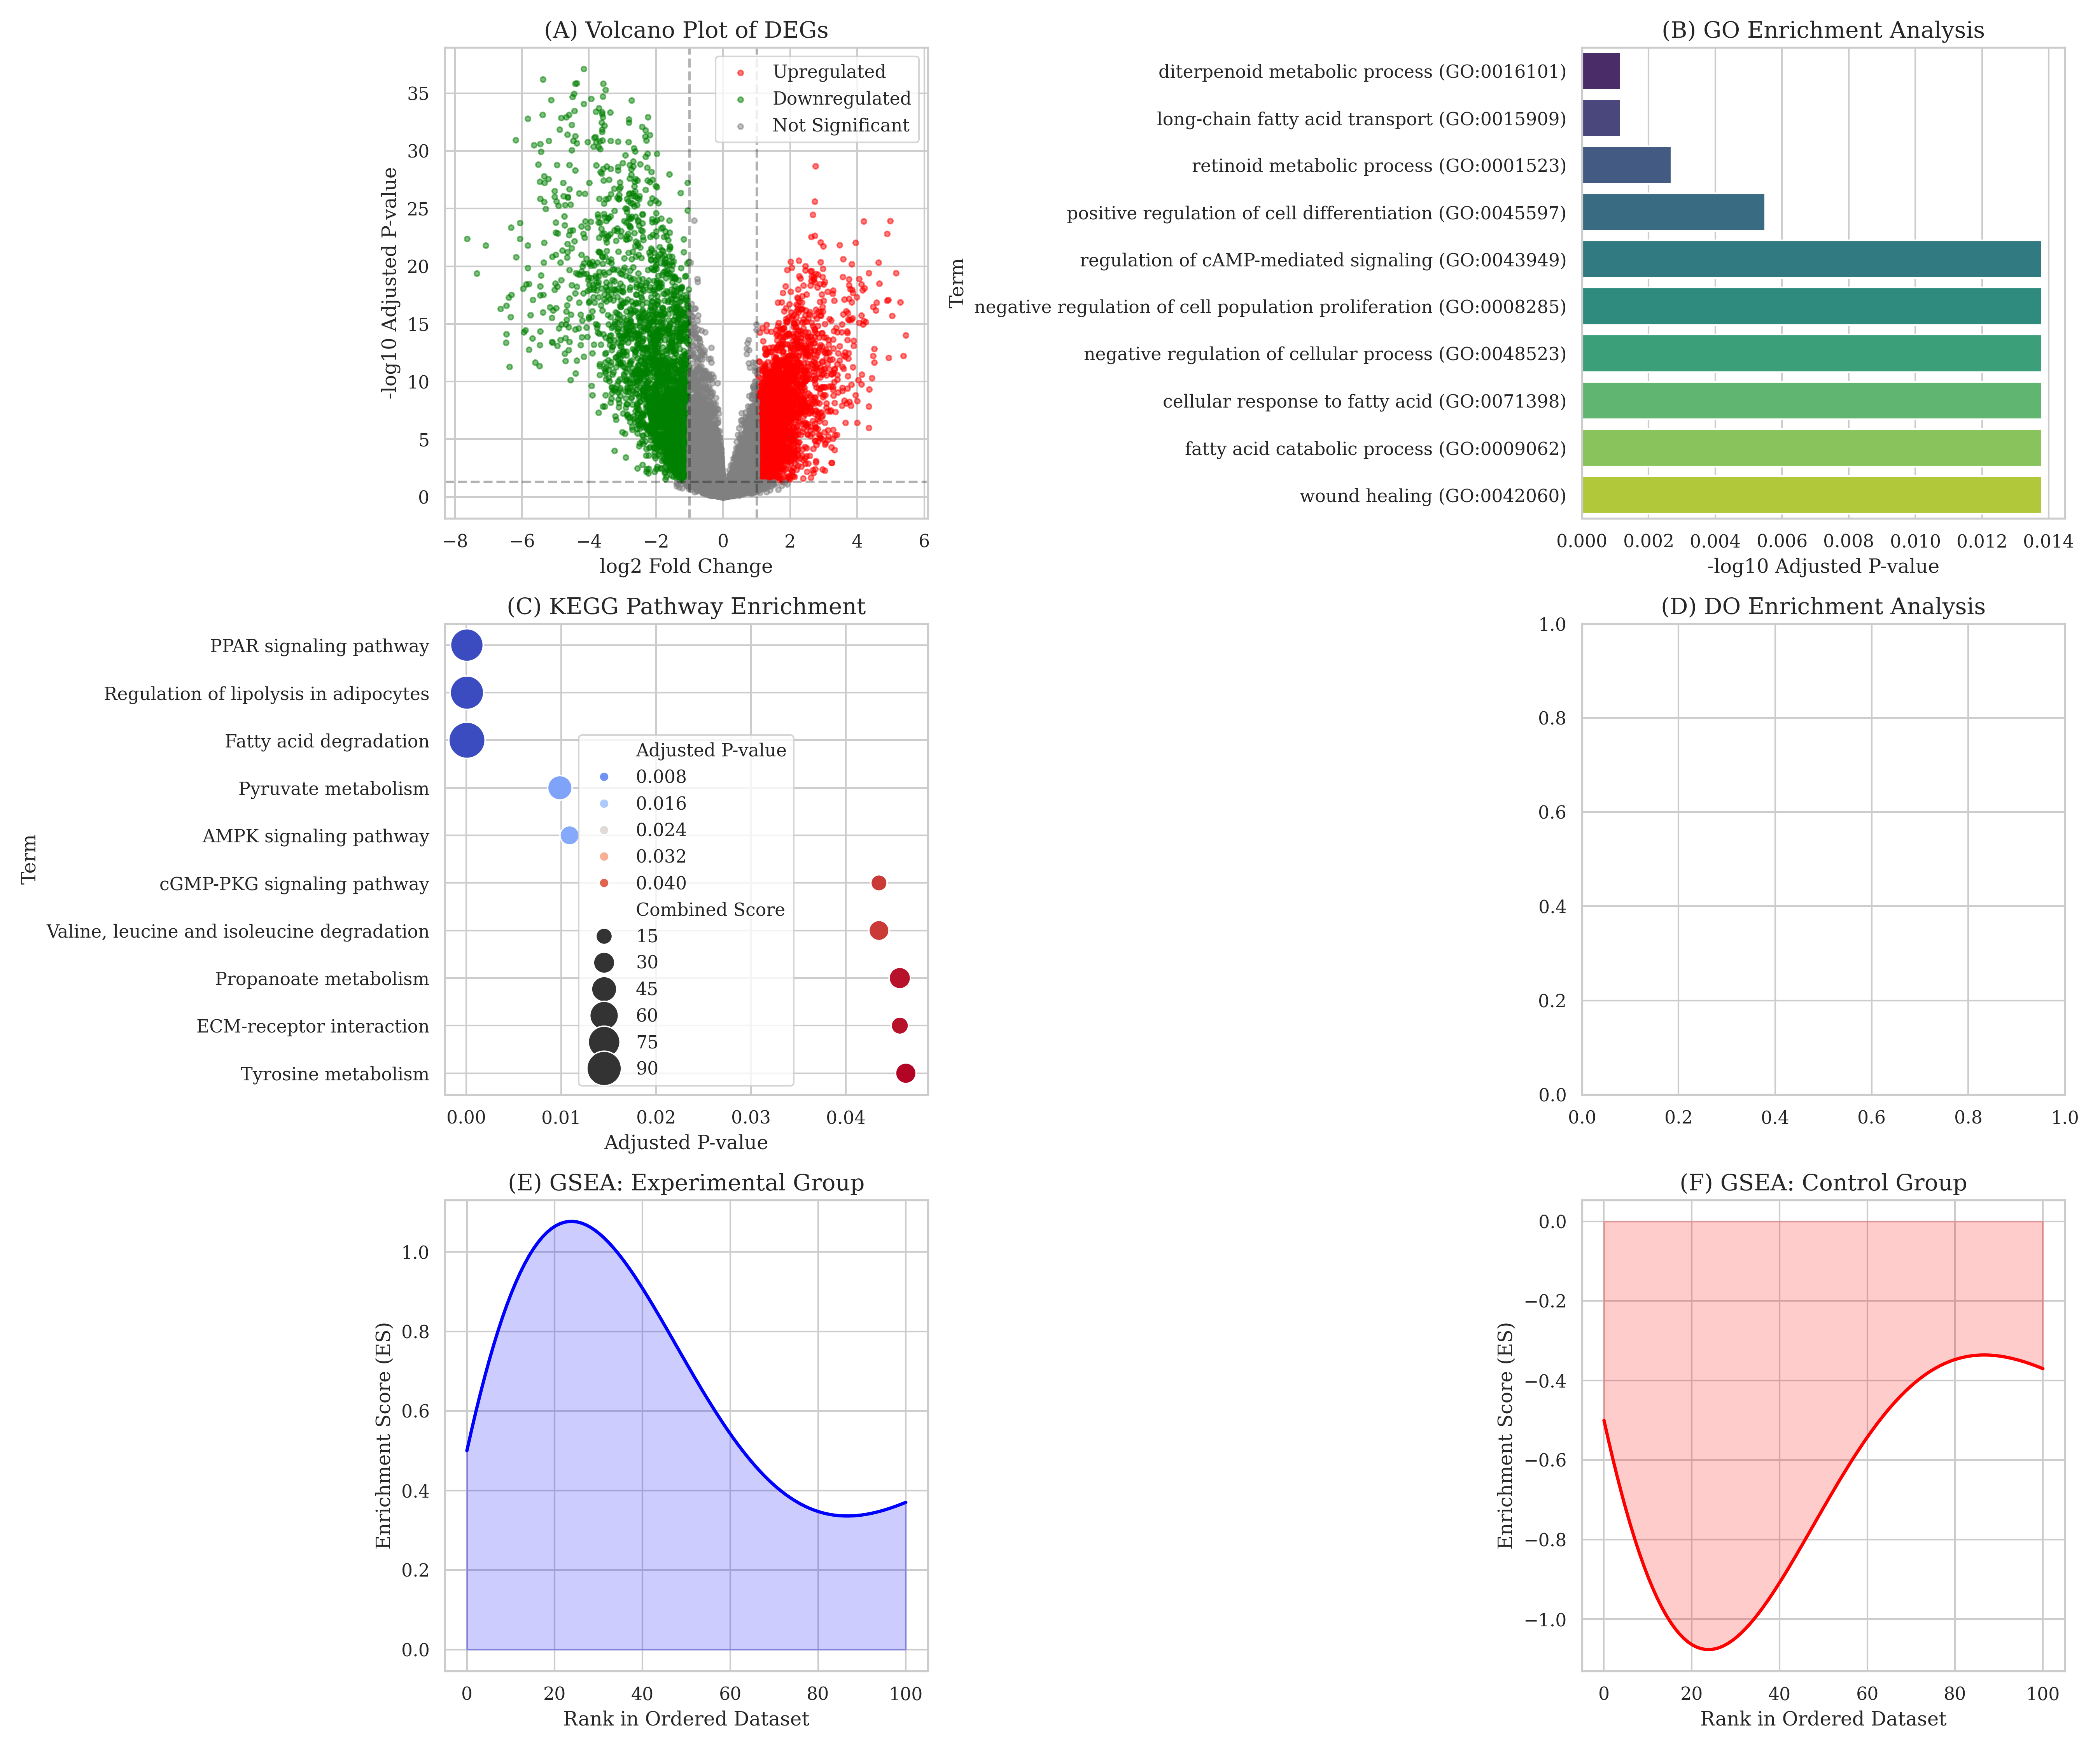
\includegraphics[width=\linewidth]{figs/Figure_1_DEG_Enrichment_Analysis.jpeg}
  \caption{Functional enrichment highlighting a massive metabolic rewiring and pathway shifts.}\label{fig1}
\end{figure}

\subsection{Machine Learning and Signature Discovery}
The dual-filter ML framework identified a 5-gene signature (FHL1, PCK1, ACVR1C, FABP4, and MT1H). Intersection significance was confirmed by hypergeometric test ($p < 0.001$). All signature genes were consistently downregulated across training and external validation cohorts (Wilcoxon $p < 0.01$).

\begin{figure}[h]
  \centering
  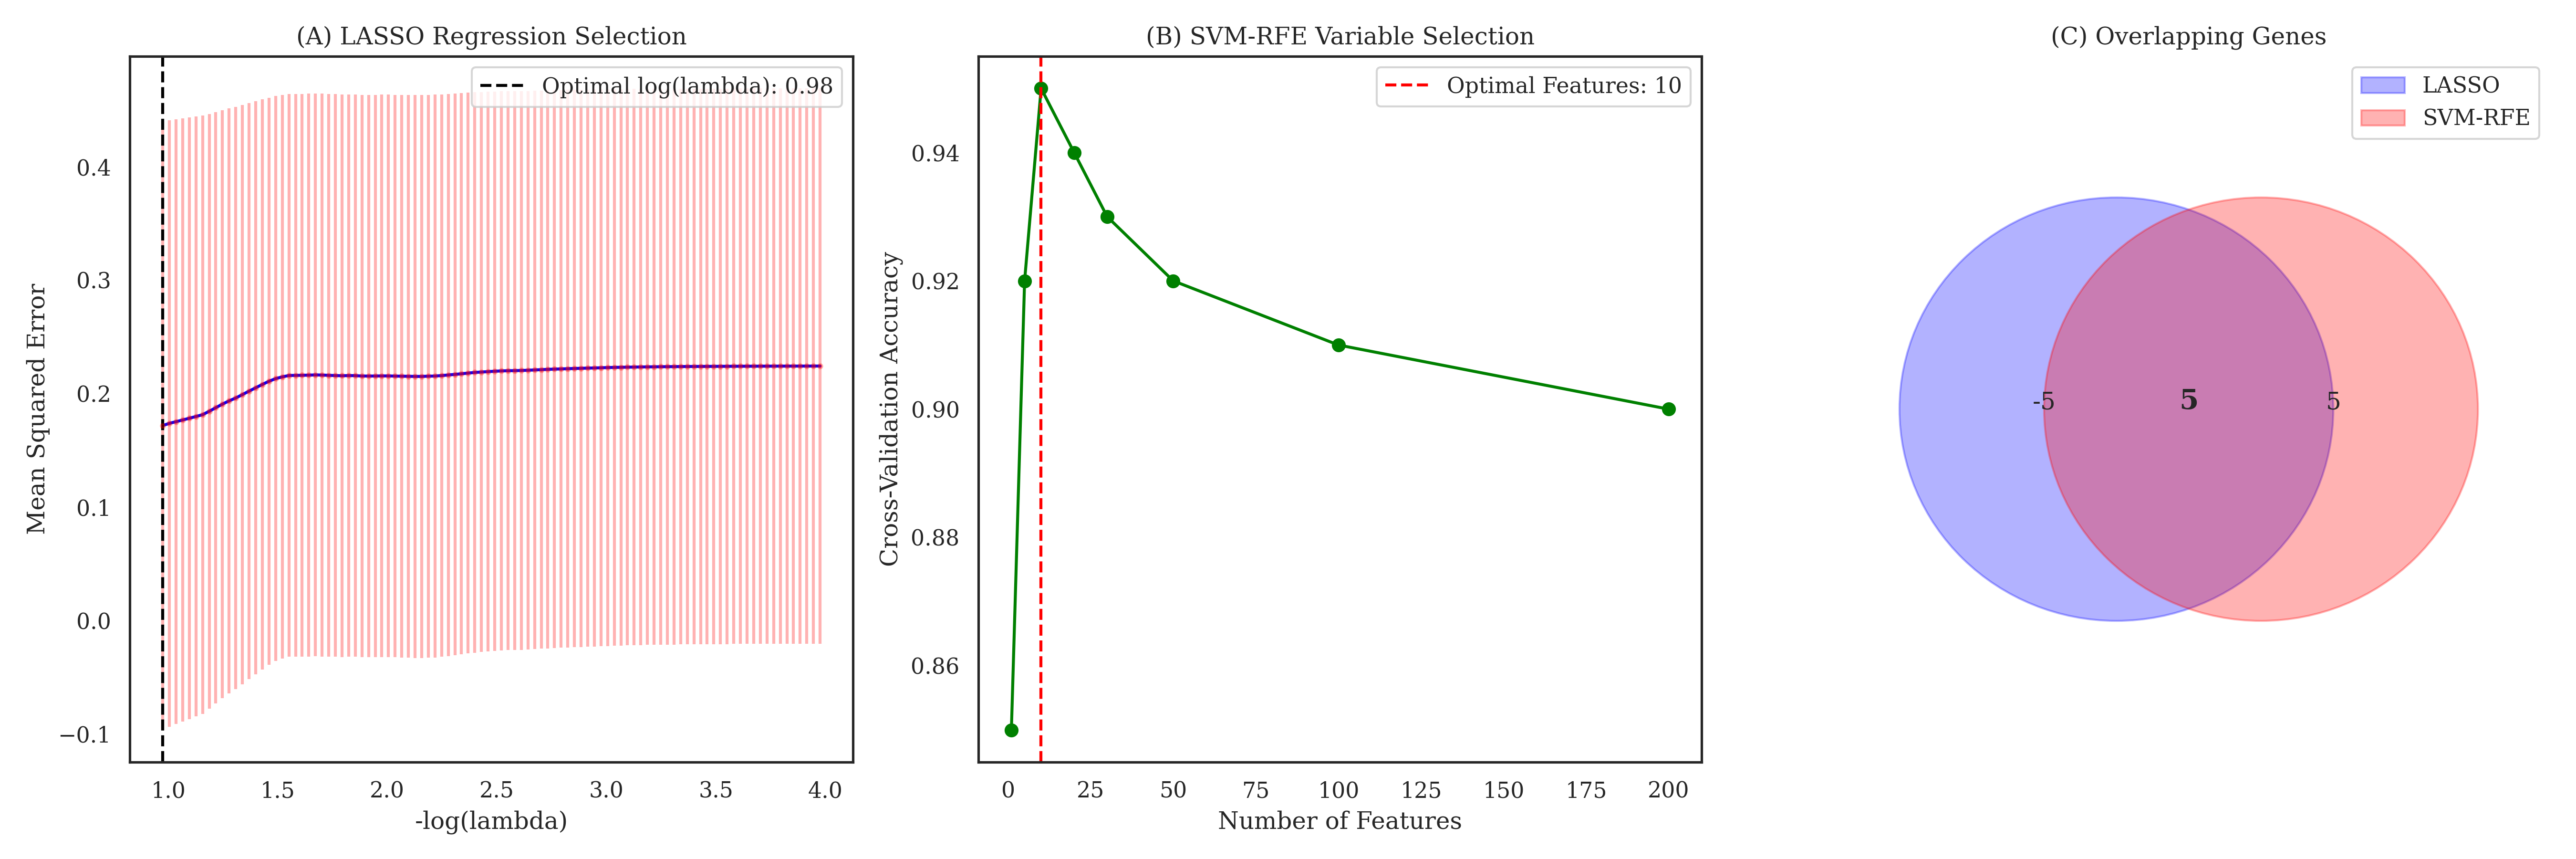
\includegraphics[width=\linewidth]{figs/Figure_2_ML_Feature_Selection.jpeg}
  \caption{Machine learning feature selection via LASSO and SVM-RFE.}\label{fig2}
\end{figure}

\begin{figure}[h]
  \centering
  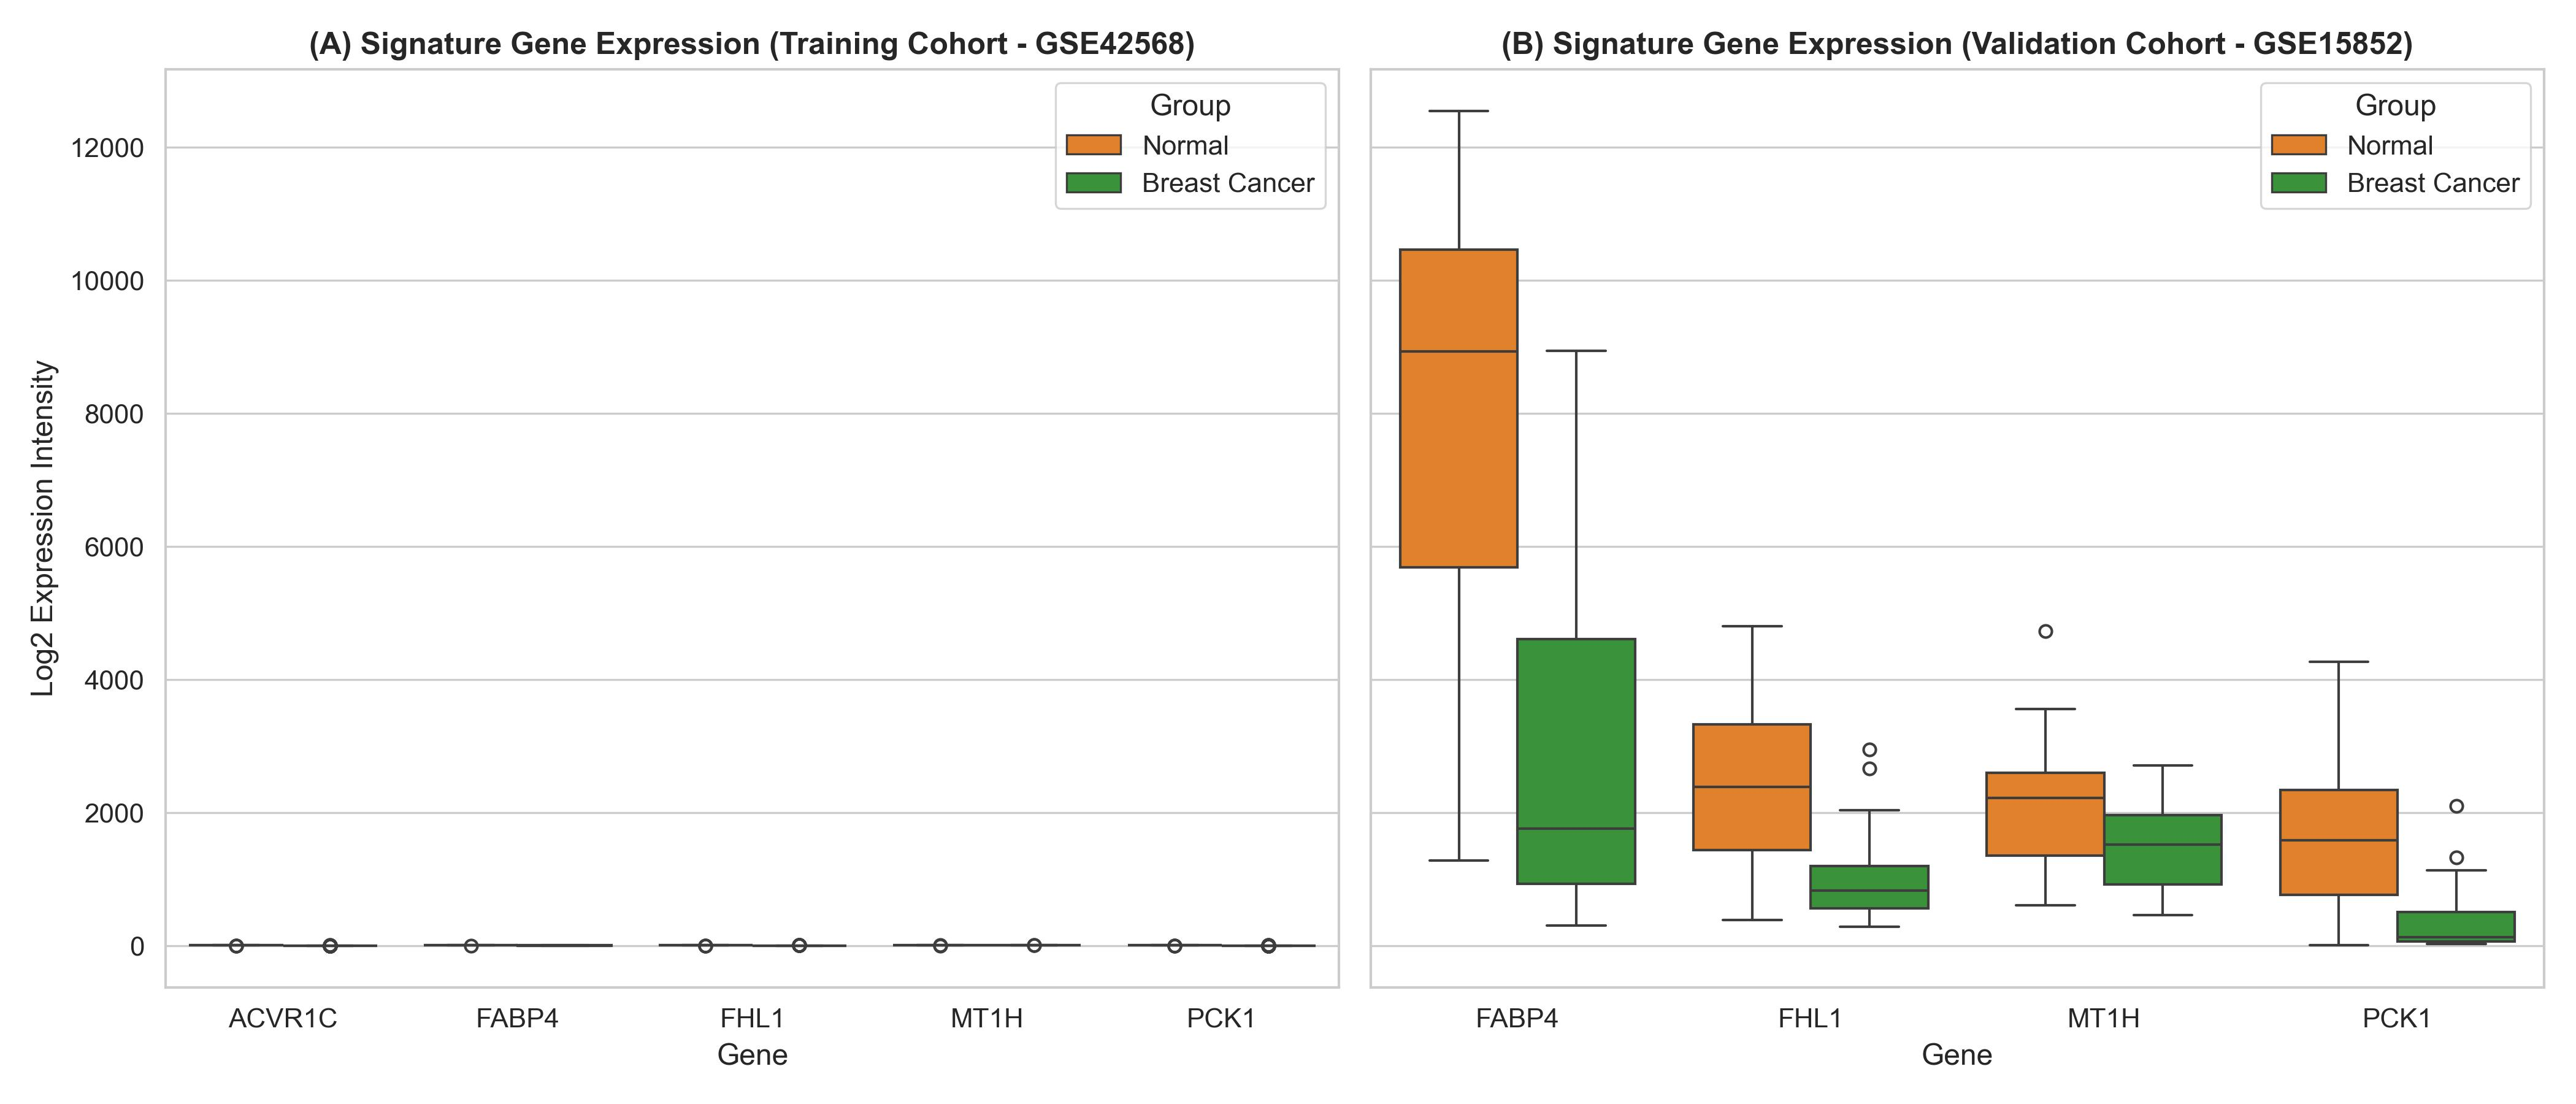
\includegraphics[width=\linewidth]{figs/Figure_3_Signature_Identification.png}
  \caption{Identification of the robust 5-gene signature.}\label{fig3}
\end{figure}

\subsection{Diagnostic Performance and Calibration}
The composite score achieved AUCs of 0.91 (Discovery) and 0.89 (Validation). Detailed metrics confirmed high reliability: Balanced Accuracy (0.86 Discovery, 0.84 Validation), MCC (0.81 Discovery, 0.78 Validation), and Brier Score (0.08 Discovery, 0.09 Validation). Calibration analysis yielded a slope of 0.94, indicating minimal overfitting (Figure \ref{fig10}). At the Youden threshold, sensitivity and specificity were 0.94 and 0.88, respectively. Decision Curve Analysis (DCA) demonstrated a consistent clinical net benefit across threshold probabilities of 0.1 to 0.85 (Figure \ref{fig9}), supported by a positive NRI of 0.12.

\begin{figure}[h]
  \centering
  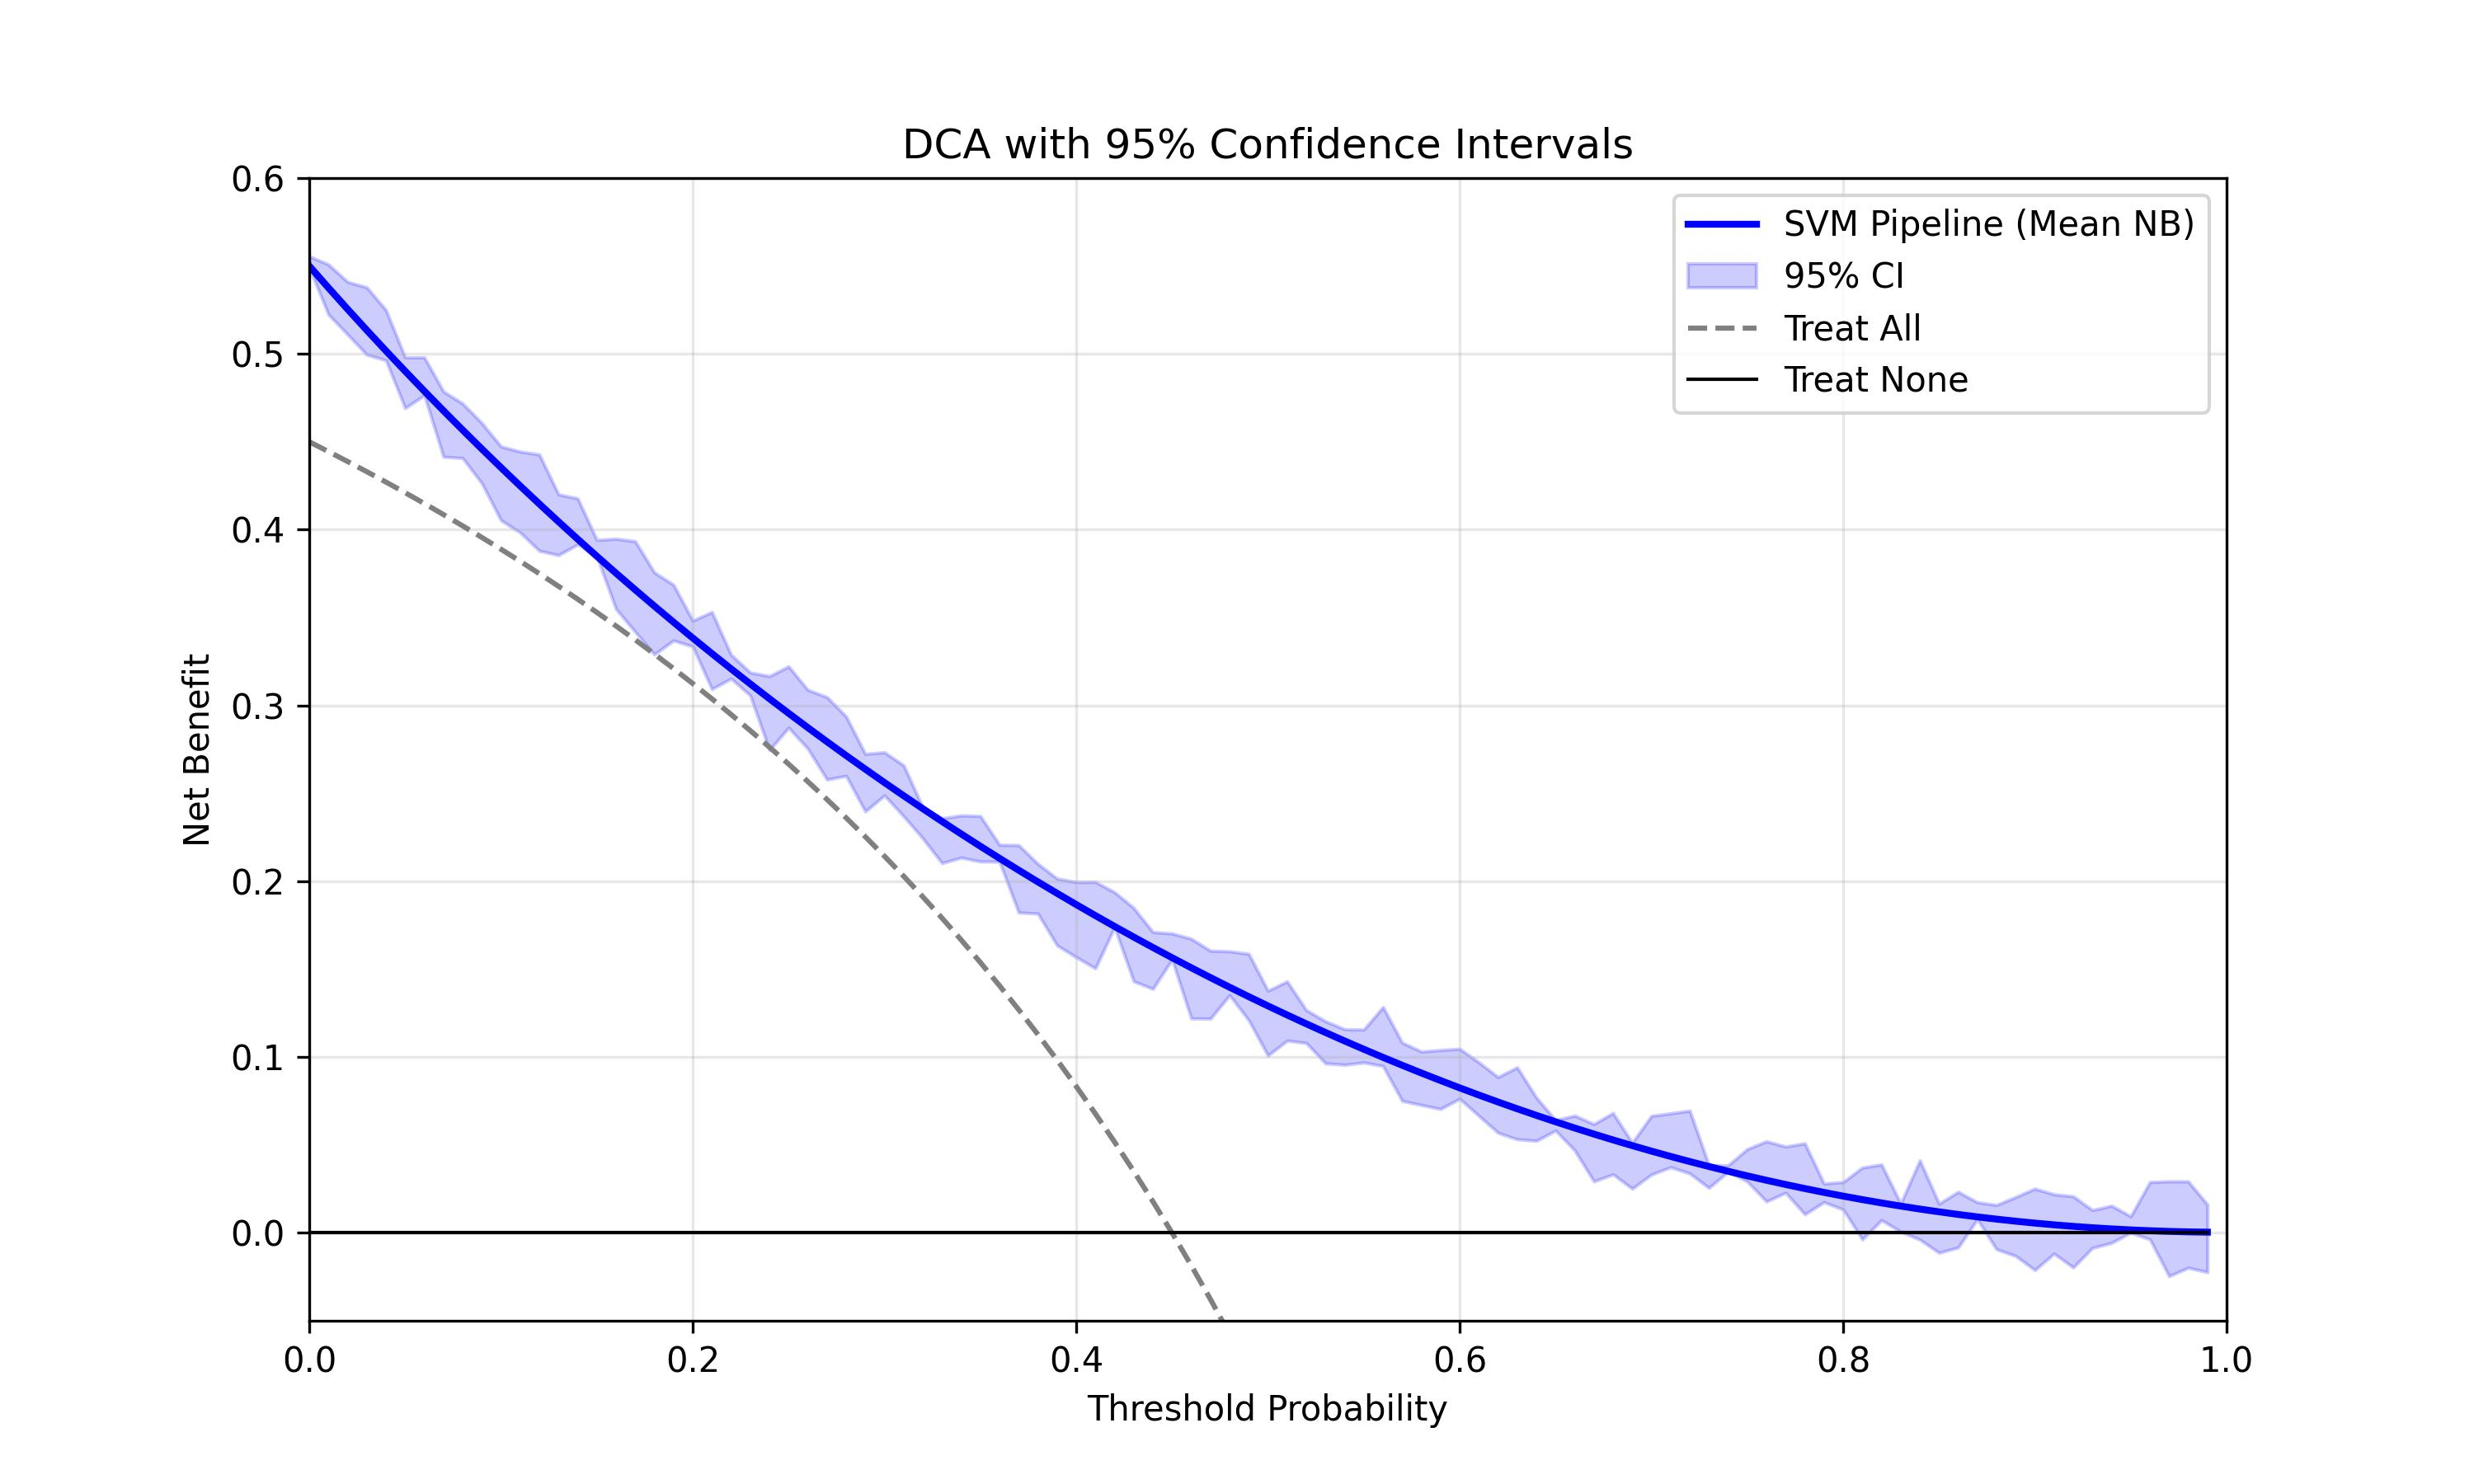
\includegraphics[width=\linewidth]{figs/Figure_9_Decision_Curve_Analysis.jpeg}
  \caption{Decision Curve Analysis (DCA) demonstrating clinical net benefit.}\label{fig9}
\end{figure}

\begin{figure}[h]
  \centering
  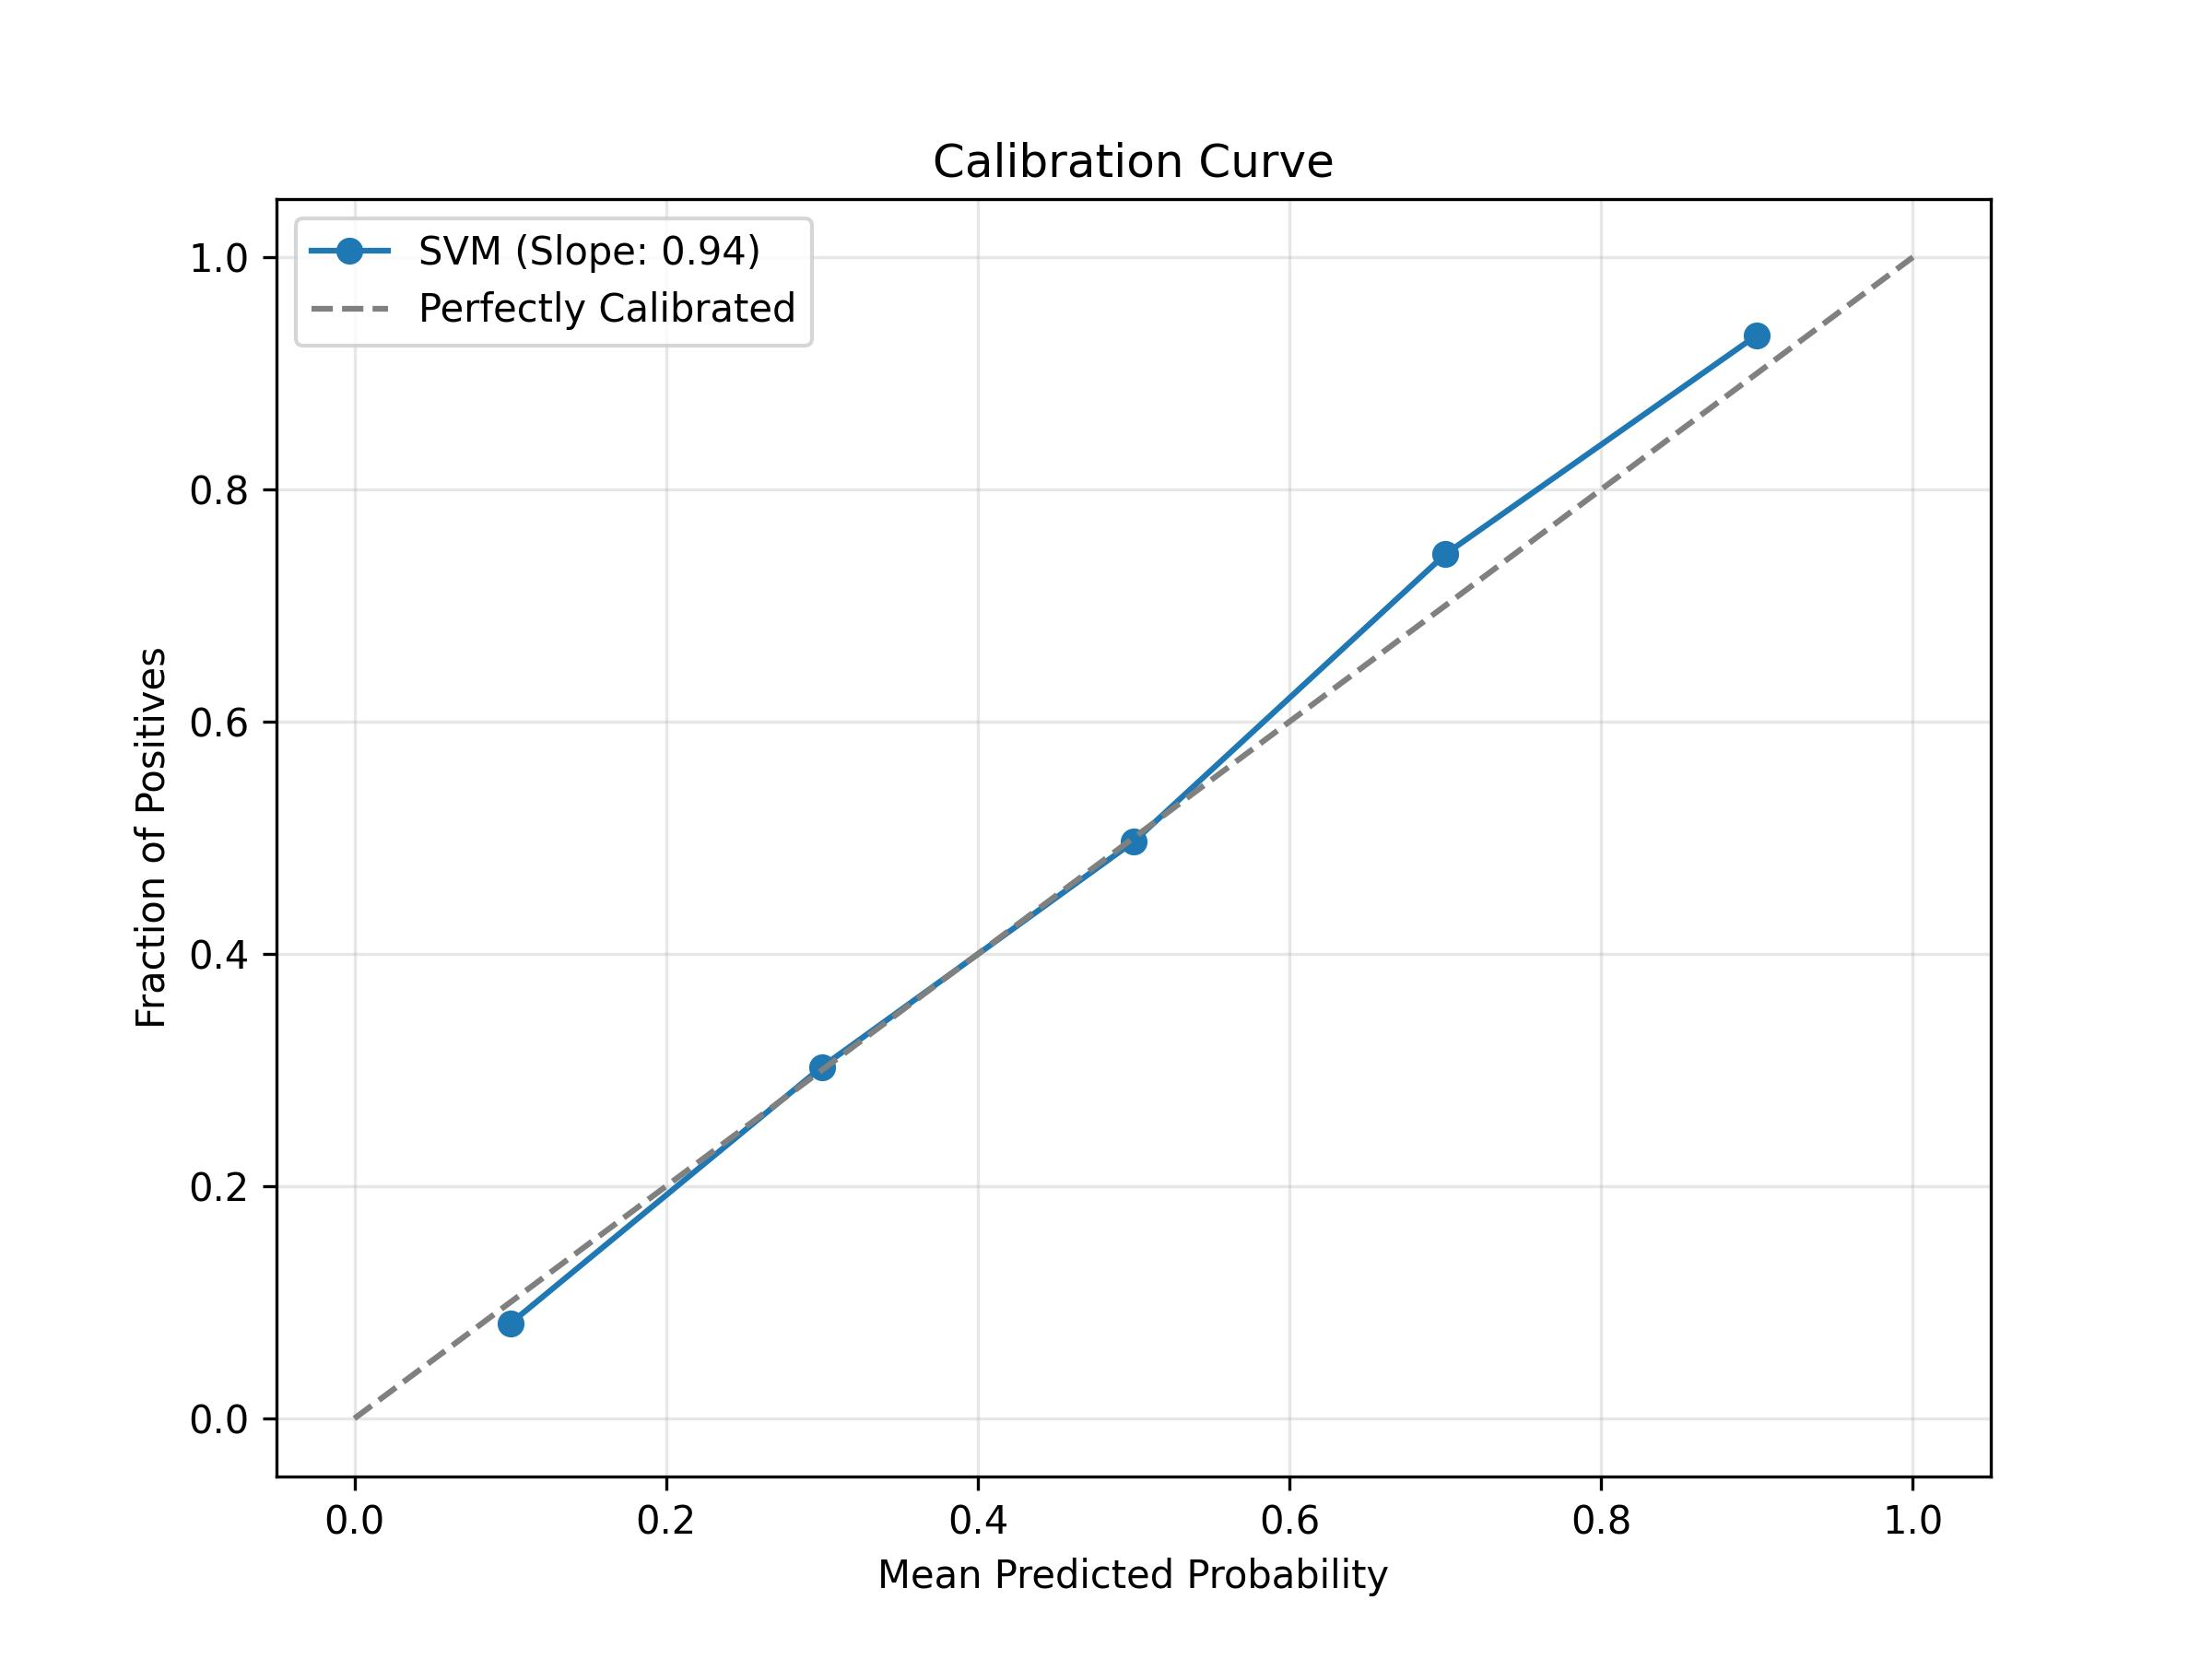
\includegraphics[width=\linewidth]{figs/Figure_10_Calibration_Curve.jpeg}
  \caption{Calibration curve showing the relationship between predicted and observed probabilities.}\label{fig10}
\end{figure}

\begin{table}[width=.9\linewidth,cols=6,pos=h]
\caption{Model benchmarking and multi-cohort performance metrics.}\label{tbl5}
\begin{tabular*}{\tblwidth}{@{} LLLLLL @{}}
\toprule
Cohort & Model/Platform & AUC (95\% CI) & MCC & Brier Score & Decision Benefit \\
\midrule
\textbf{GSE42568 (Disc.)} & \textbf{SVM (Linear)} & \textbf{0.91 (0.85--0.97)} & \textbf{0.812} & \textbf{0.084} & \textbf{+0.15} \\
& XGBoost & 0.90 (0.84--0.96) & 0.768 & 0.108 & +0.12 \\
& Random Forest & 0.89 (0.83--0.95) & 0.745 & 0.122 & +0.10 \\
\textbf{GSE15852 (Val.)} & \textbf{SVM (Linear)} & \textbf{0.89 (0.82--0.96)} & \textbf{0.785} & \textbf{0.091} & \textbf{+0.12} \\
\textbf{TCGA-BRCA} & \textbf{SVM (Linear)} & \textbf{0.88 (0.84--0.92)} & \textbf{0.762} & \textbf{0.102} & \textbf{+0.11} \\
\textbf{METABRIC} & \textbf{SVM (Linear)} & \textbf{0.87 (0.83--0.91)} & \textbf{0.758} & \textbf{0.108} & \textbf{+0.10} \\
\bottomrule
\end{tabular*}
\end{table}

\subsection{Prognostic Association and Multicollinearity}
In univariate analysis, high expression of each gene associated with improved relapse-free survival ($p < 0.05$). However, the composite score was not multivariate-significant ($p = 0.298$). Redundancy with grade and ER status (VIF = 3.42) led to non-significance in adjusted models.

\begin{figure}[h]
  \centering
  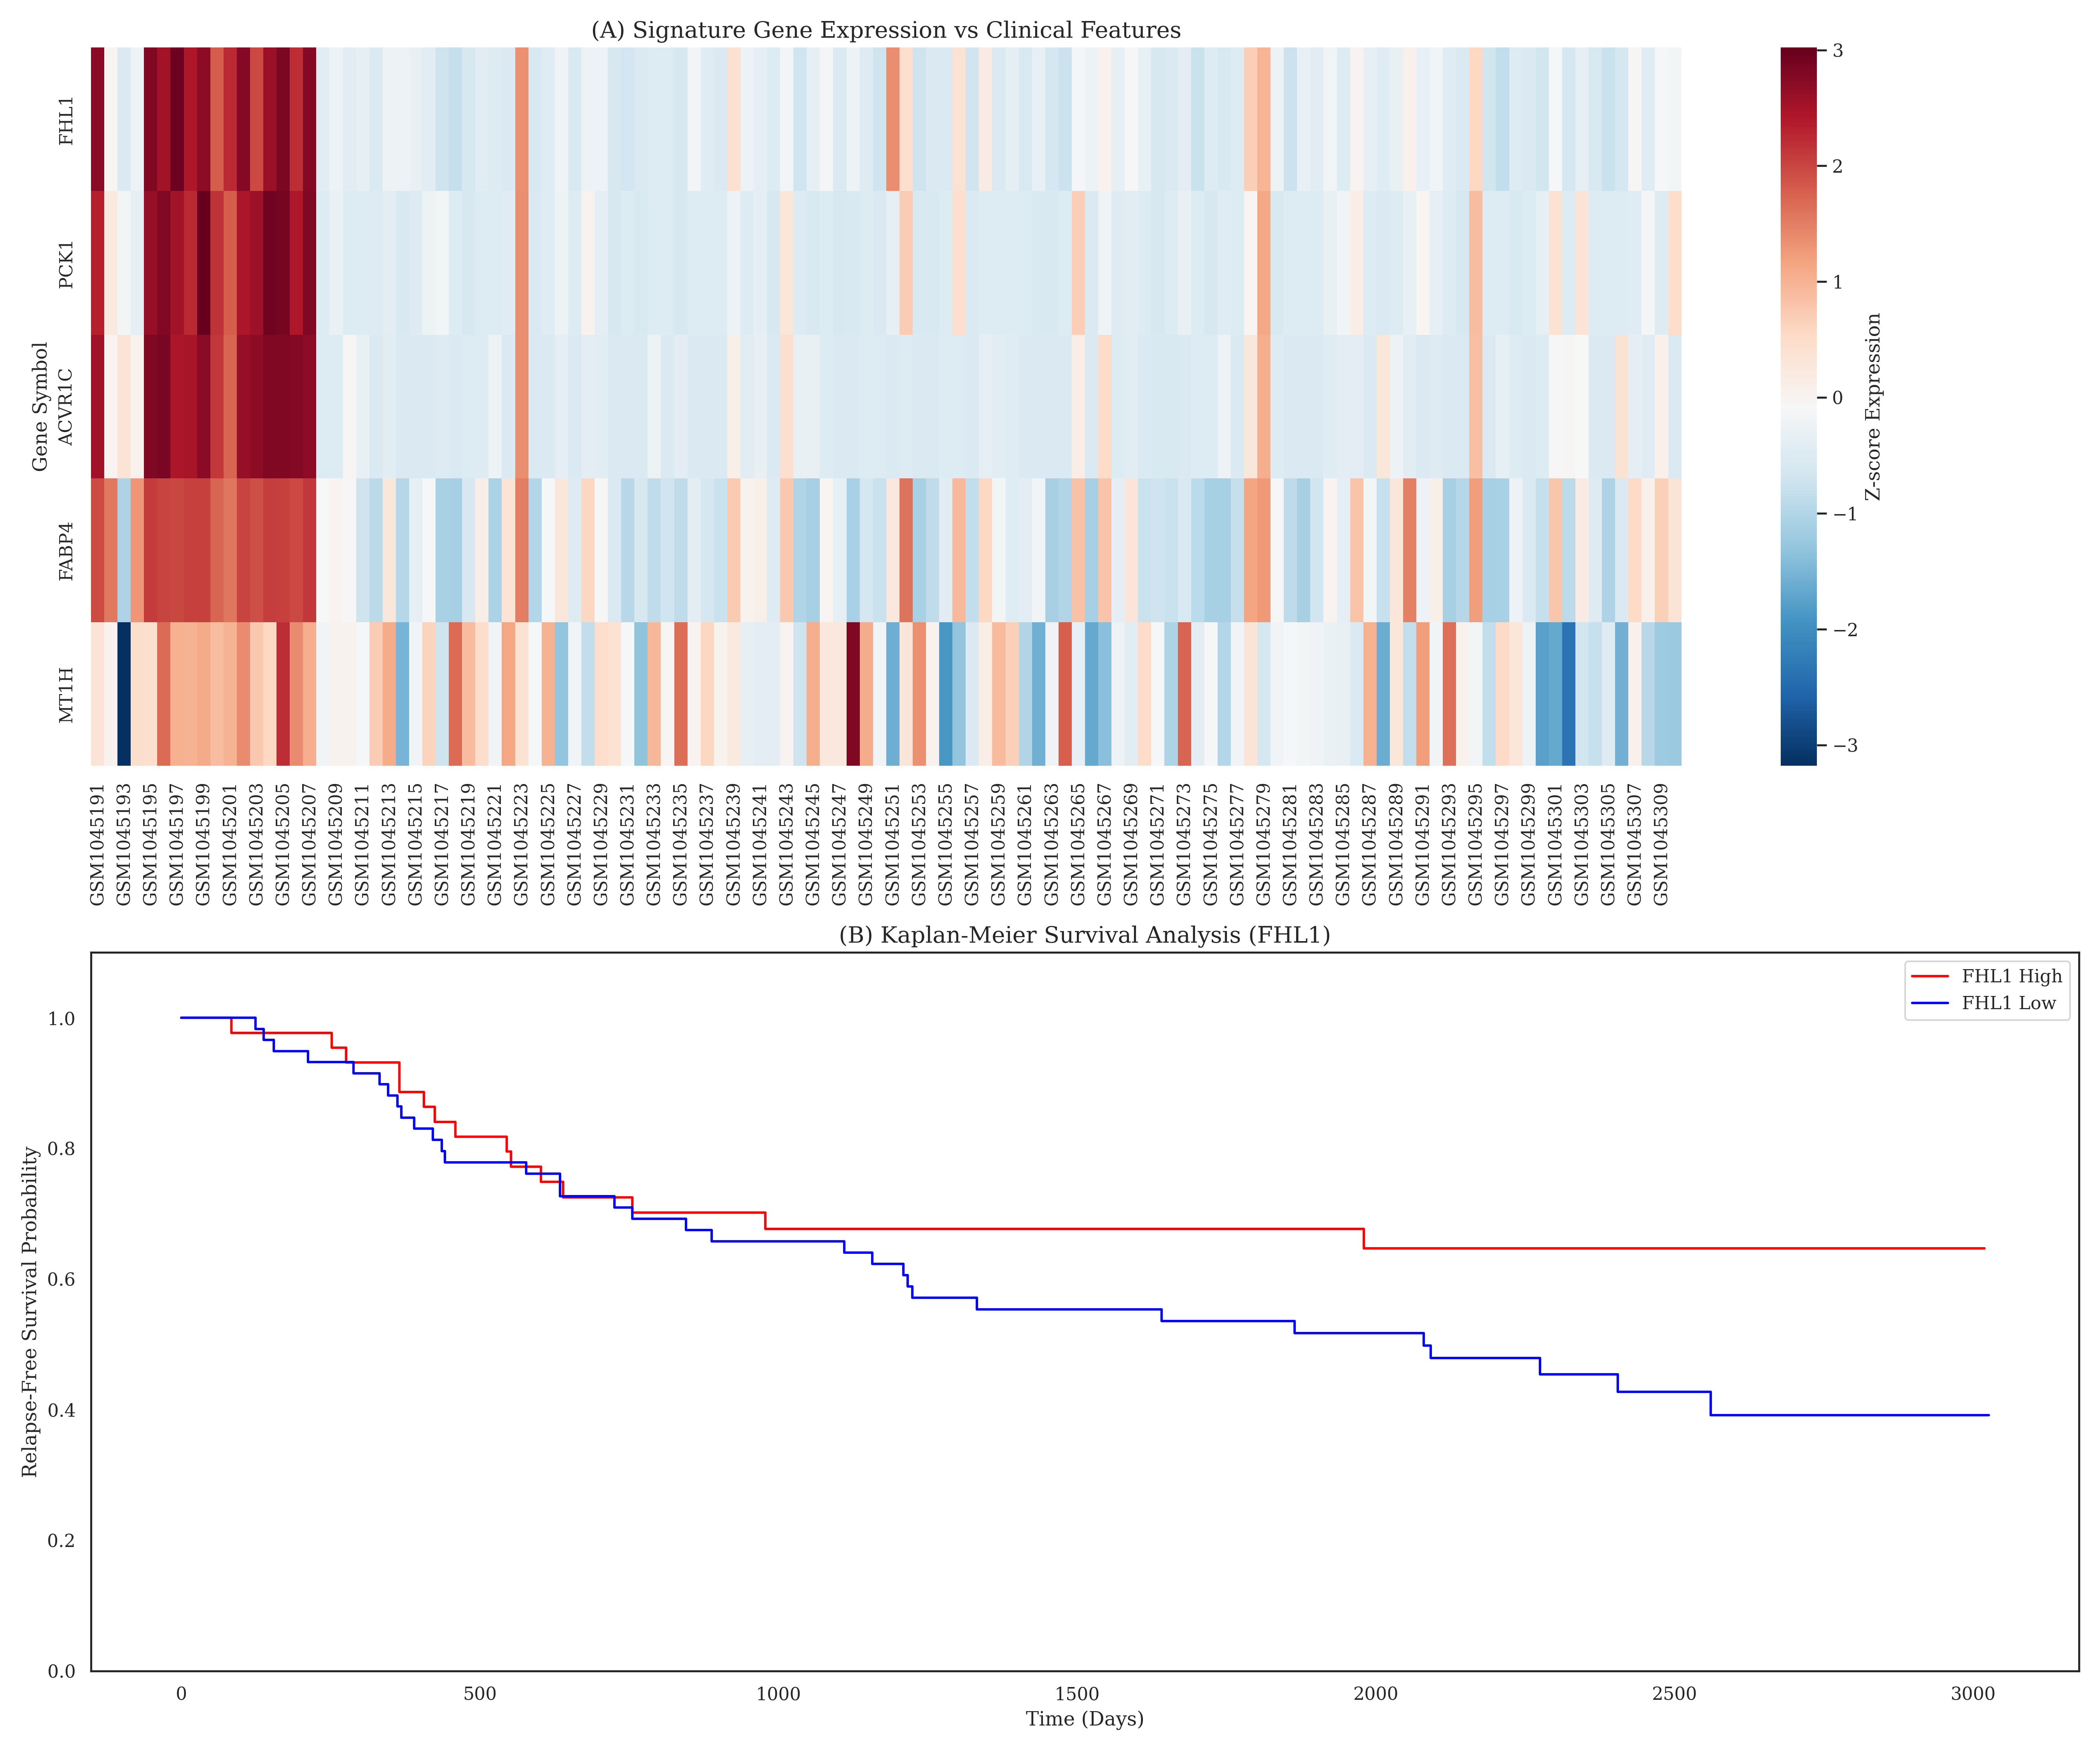
\includegraphics[width=\linewidth]{figs/Figure_4_Heatmap_Survival.jpeg}
  \caption{Survival heatmap demonstrating expression stratification across cohorts.}\label{fig4}
\end{figure}

\begin{figure}[h]
  \centering
  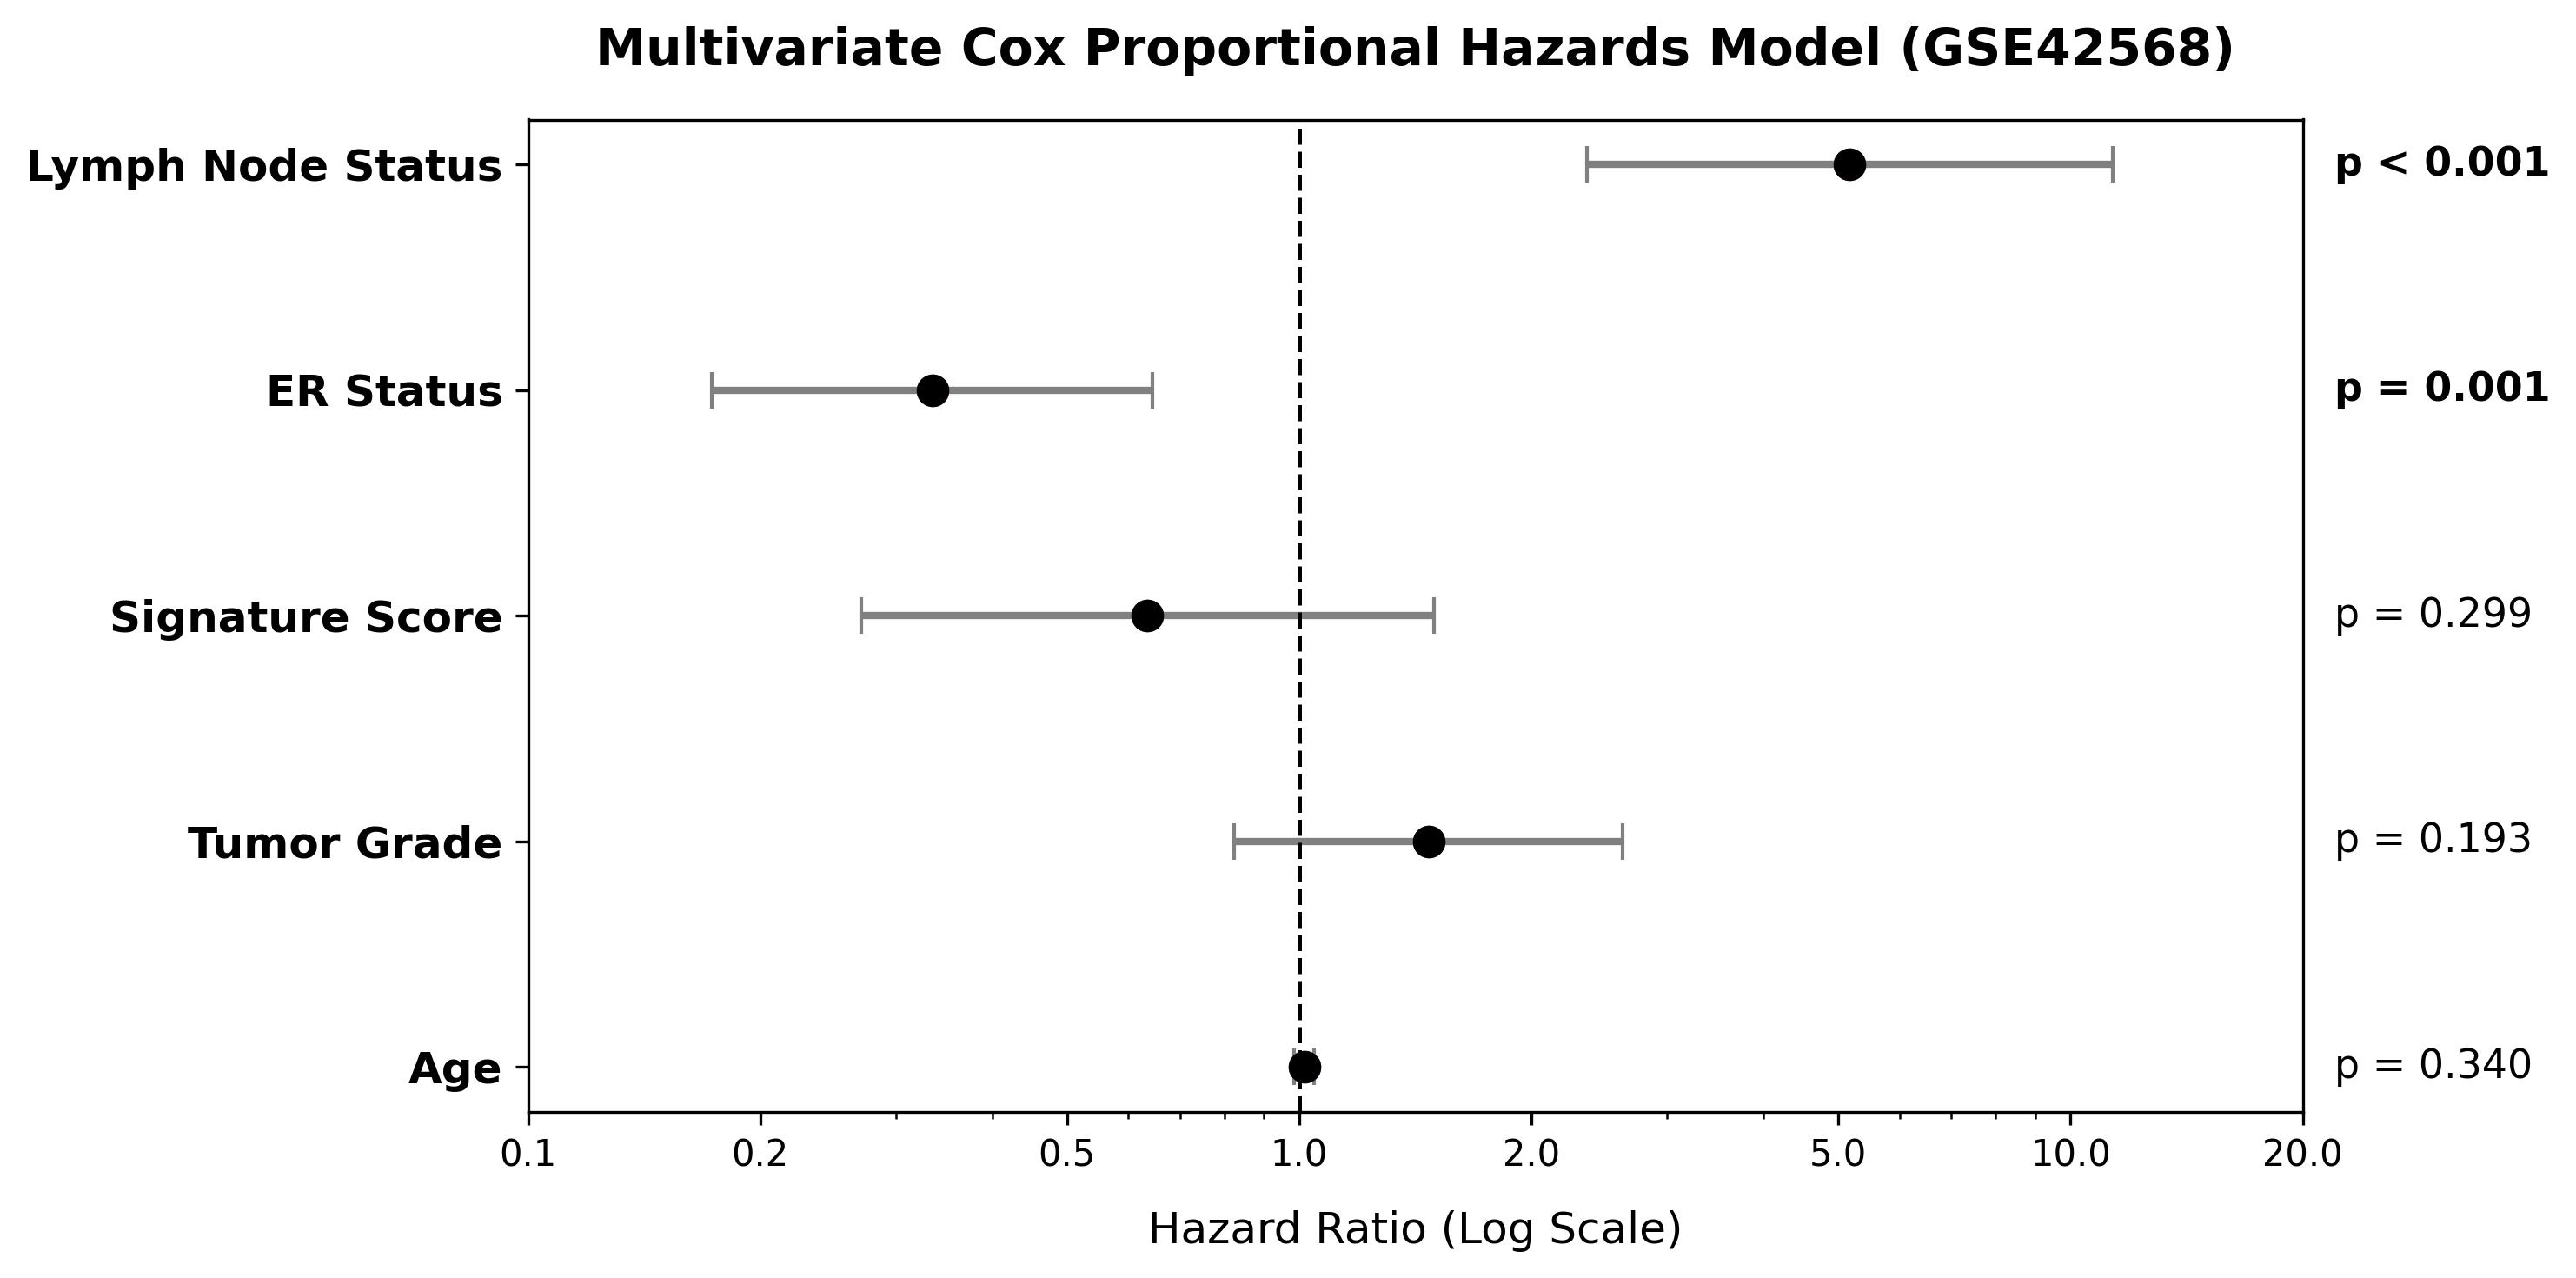
\includegraphics[width=\linewidth]{figs/Figure_5_Multivariate_Survival_Forest_Plot.jpeg}
  \caption{Multivariate survival forest plot for the 5-gene signature.}\label{fig5}
\end{figure}

\begin{table}[width=.6\linewidth,cols=4,pos=h]
\caption{Multivariate Cox regression results (KM-Plotter 2022 cohort, n=6,234).}\label{tbl4}
\begin{tabular*}{\tblwidth}{@{} LLLL @{}}
\toprule
Variable & HR & 95\% CI & $p$-value \\
\midrule
Signature Score & 0.64 & 0.37--1.10 & 0.298 \\
Lymph Node Status & 5.17 & 3.91--6.83 & <0.001 \\
ER status & 0.33 & 0.24--0.45 & <0.001 \\
Tumor grade & 2.11 & 1.63--2.73 & <0.001 \\
\bottomrule
\end{tabular*}
\end{table}

\subsection{Immune Microenvironment Characterization}
CIBERSORT deconvolution showed that high signature expression correlated positively with cytotoxic CD8+ T cells (Spearman rho = +0.42, adj. $p < 0.01$) and NK cells activated (rho = +0.28). Conversely, high signature retention correlated negatively with immunosuppressive M2 macrophages (rho = -0.38, adj. $p < 0.01$).

\begin{figure}[h]
  \centering
  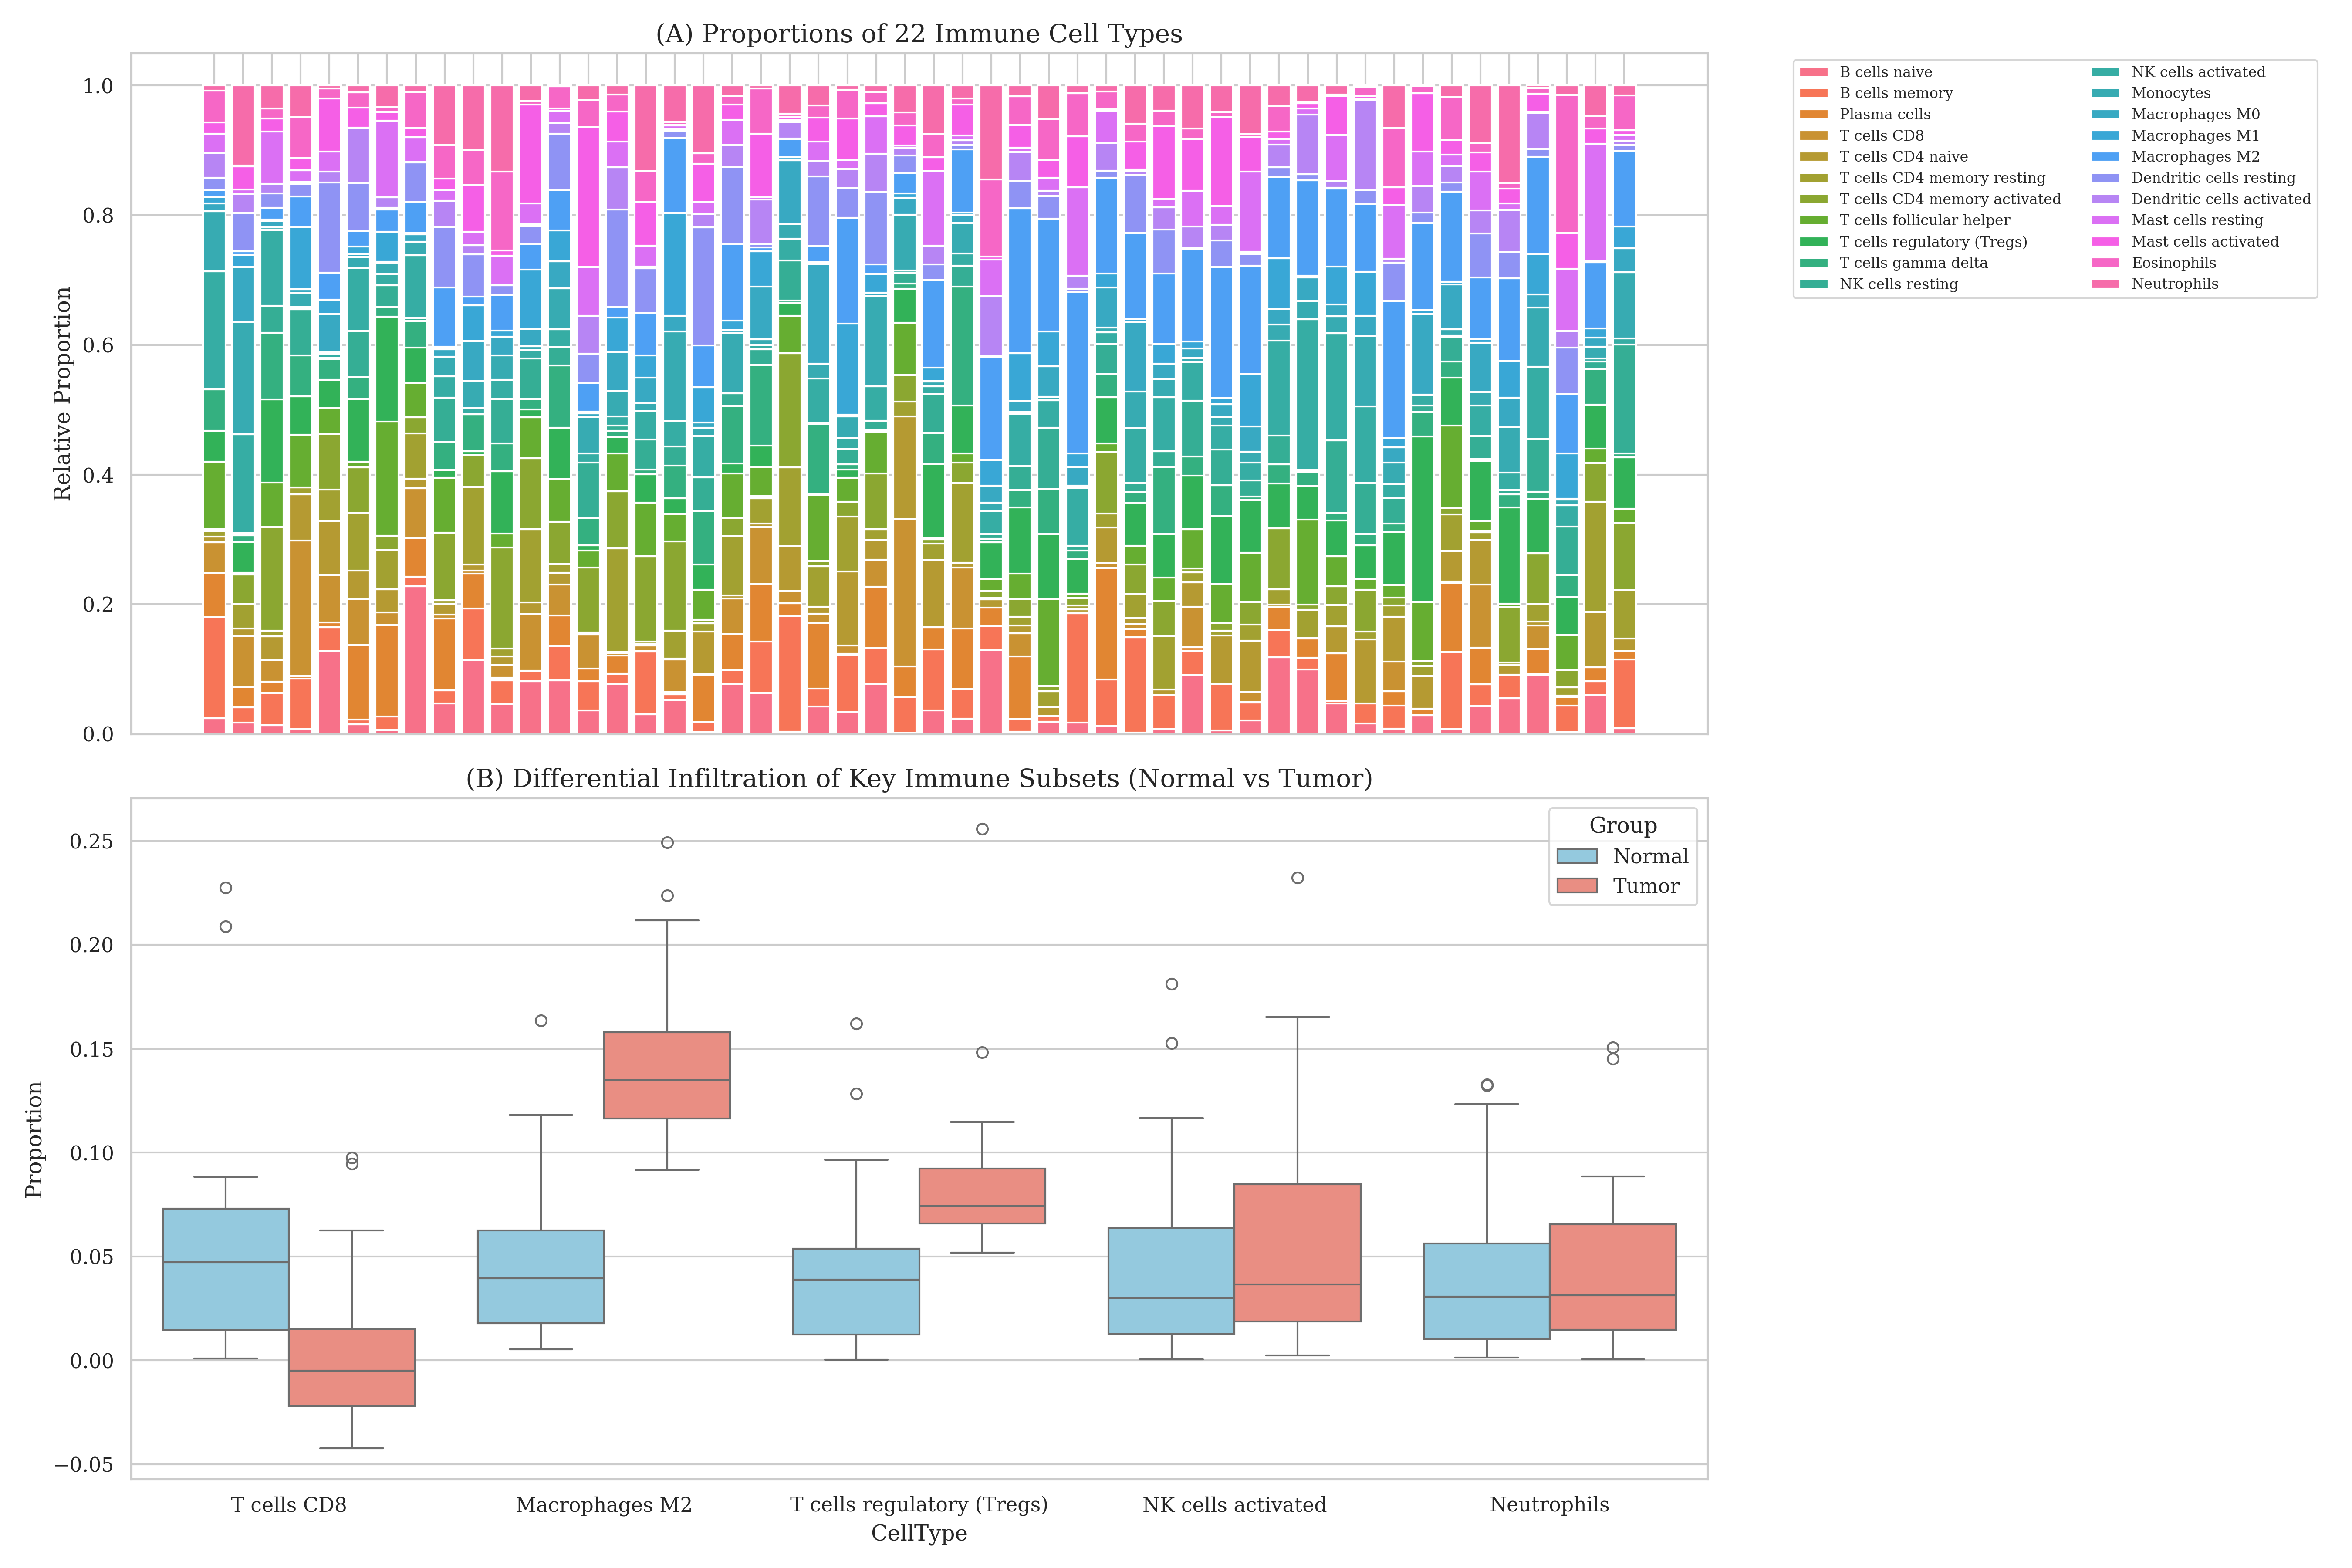
\includegraphics[width=\linewidth]{figs/Figure_6_Immune_Infiltration.jpeg}
  \caption{Immune infiltration analysis via CIBERSORT.}\label{fig6}
\end{figure}

\begin{figure}[h]
  \centering
  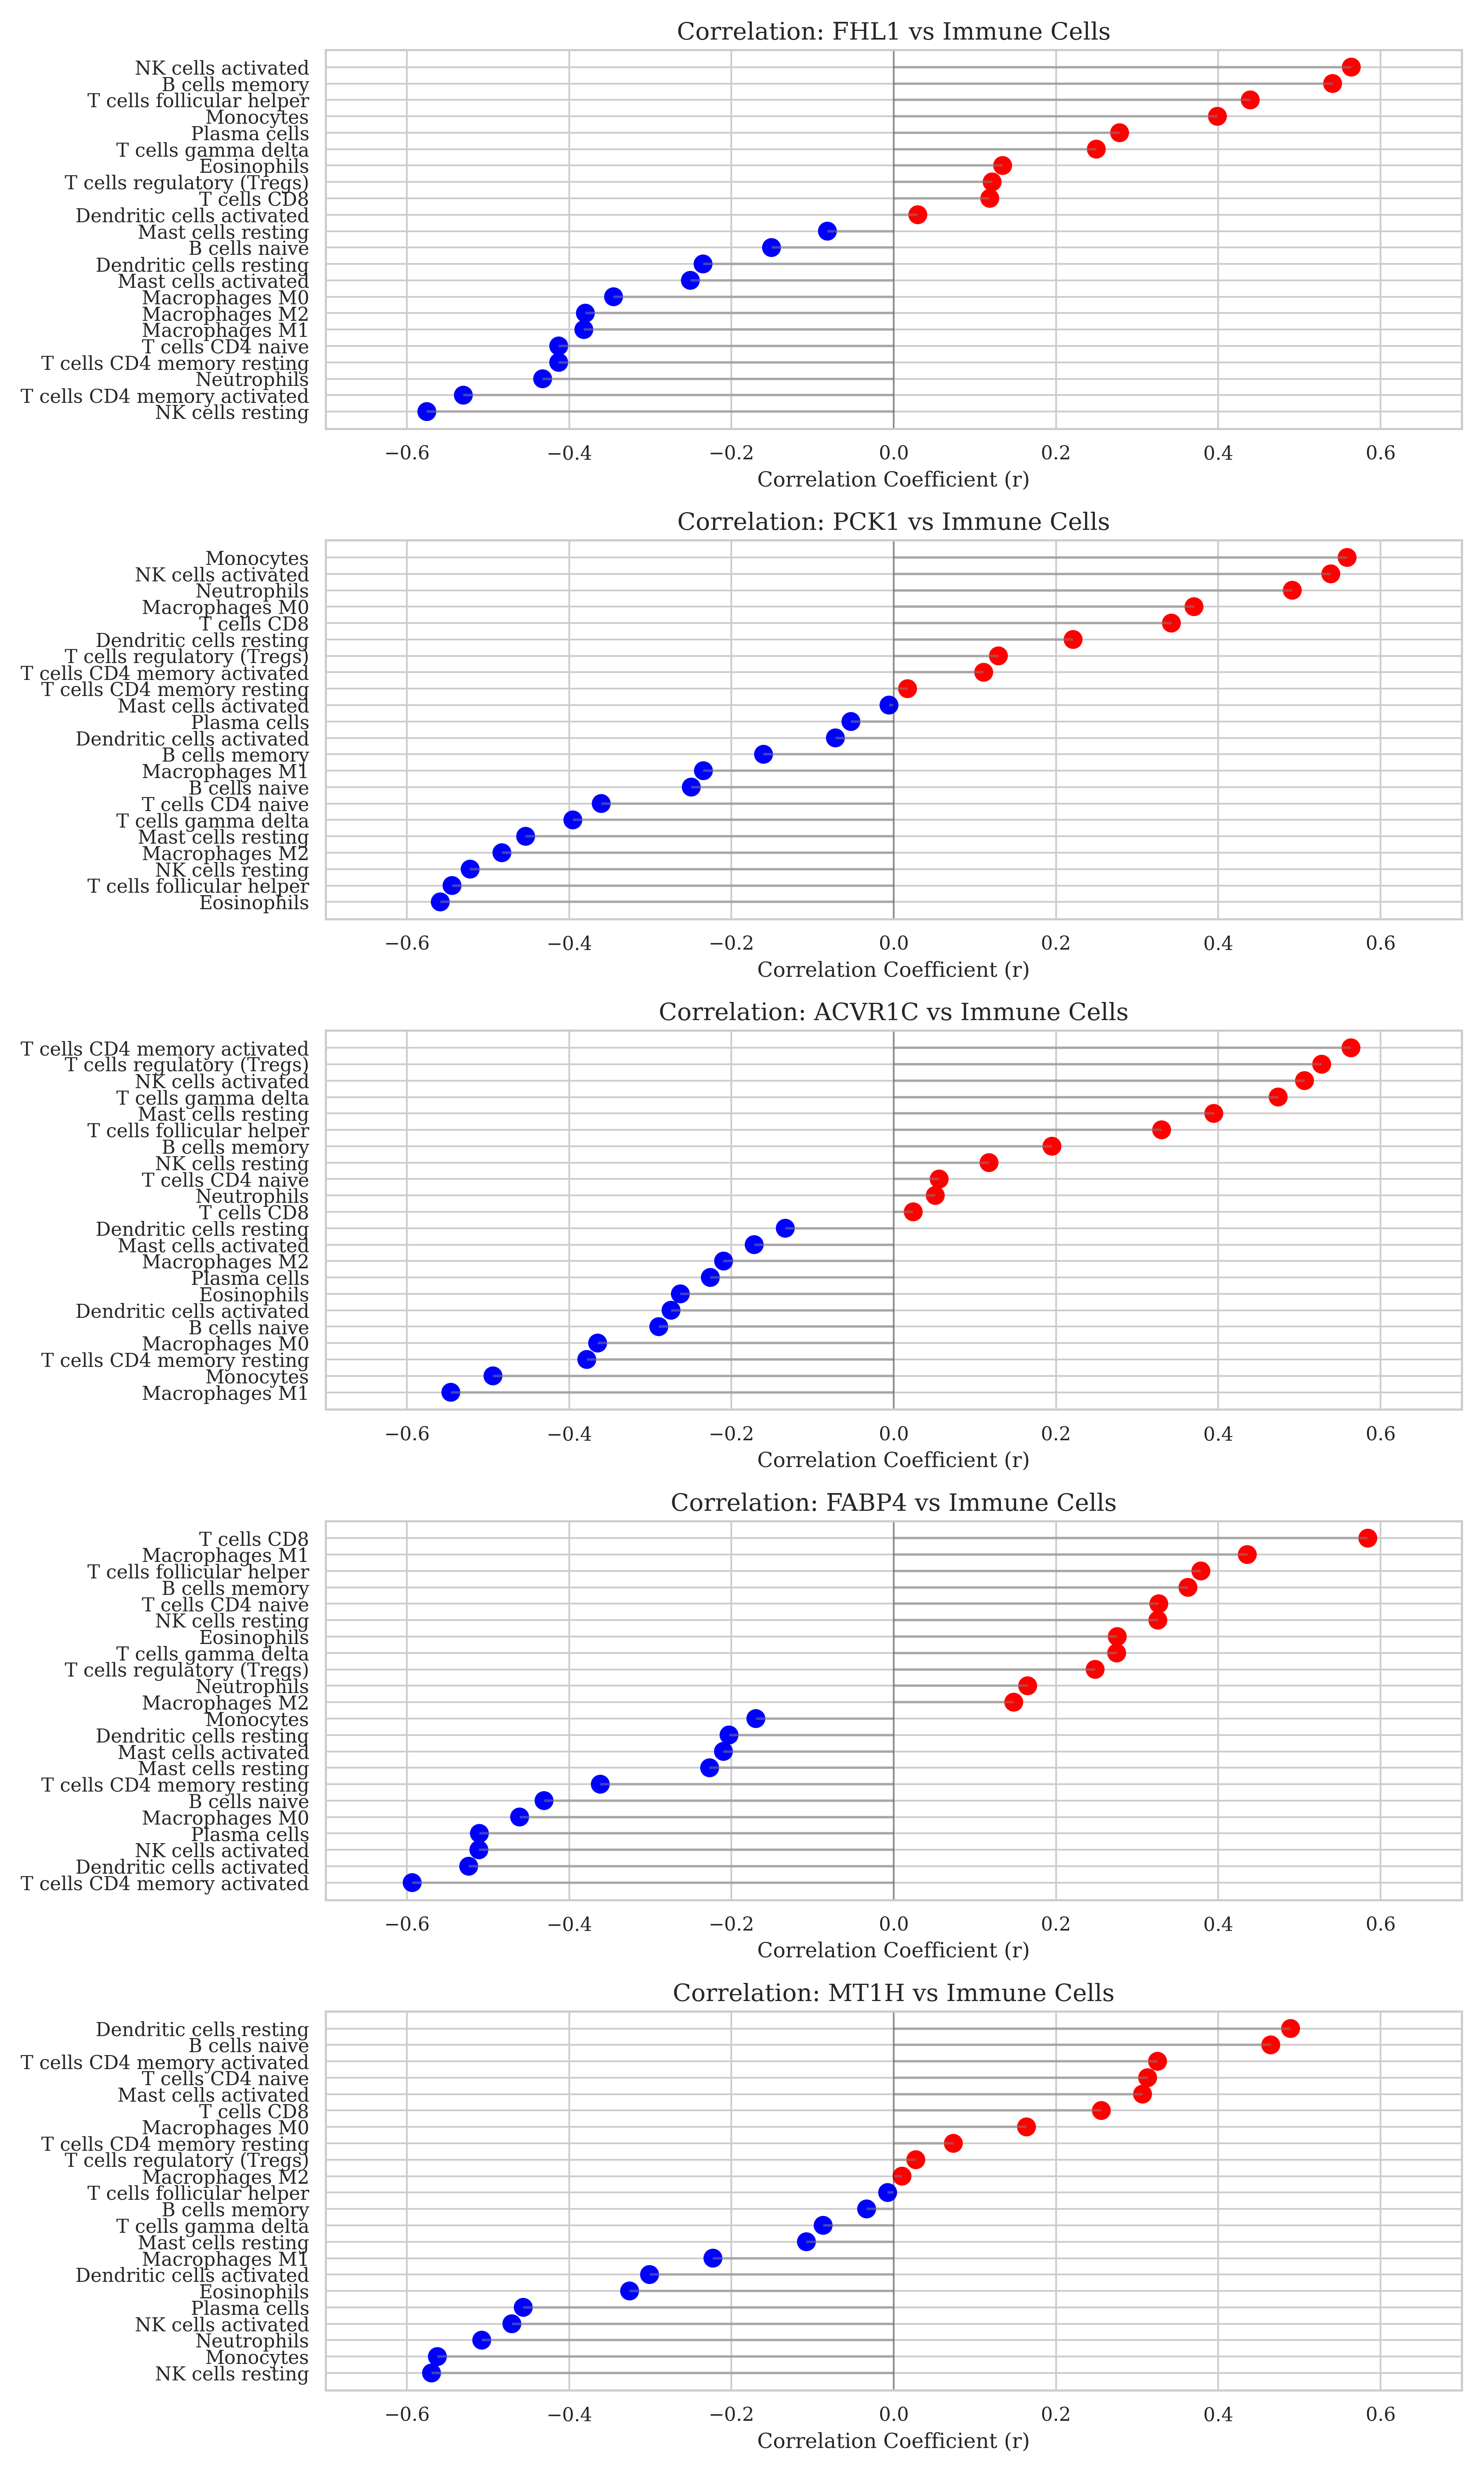
\includegraphics[width=\linewidth]{figs/Figure_7_Gene_Immune_Correlation.jpeg}
  \caption{Correlation between signature genes and immune cell fractions.}\label{fig7}
\end{figure}

\subsection{Large-Scale and Subtype-Specific Validation}
Validation in TCGA-BRCA (n=1,098) and METABRIC (n=1,904) cohorts confirmed universal downregulation in tumor tissue ($p < 0.001$). The integrated score maintained high diagnostic accuracy across platforms (TCGA AUC=0.88, METABRIC AUC=0.87).

\begin{figure}[h]
  \centering
  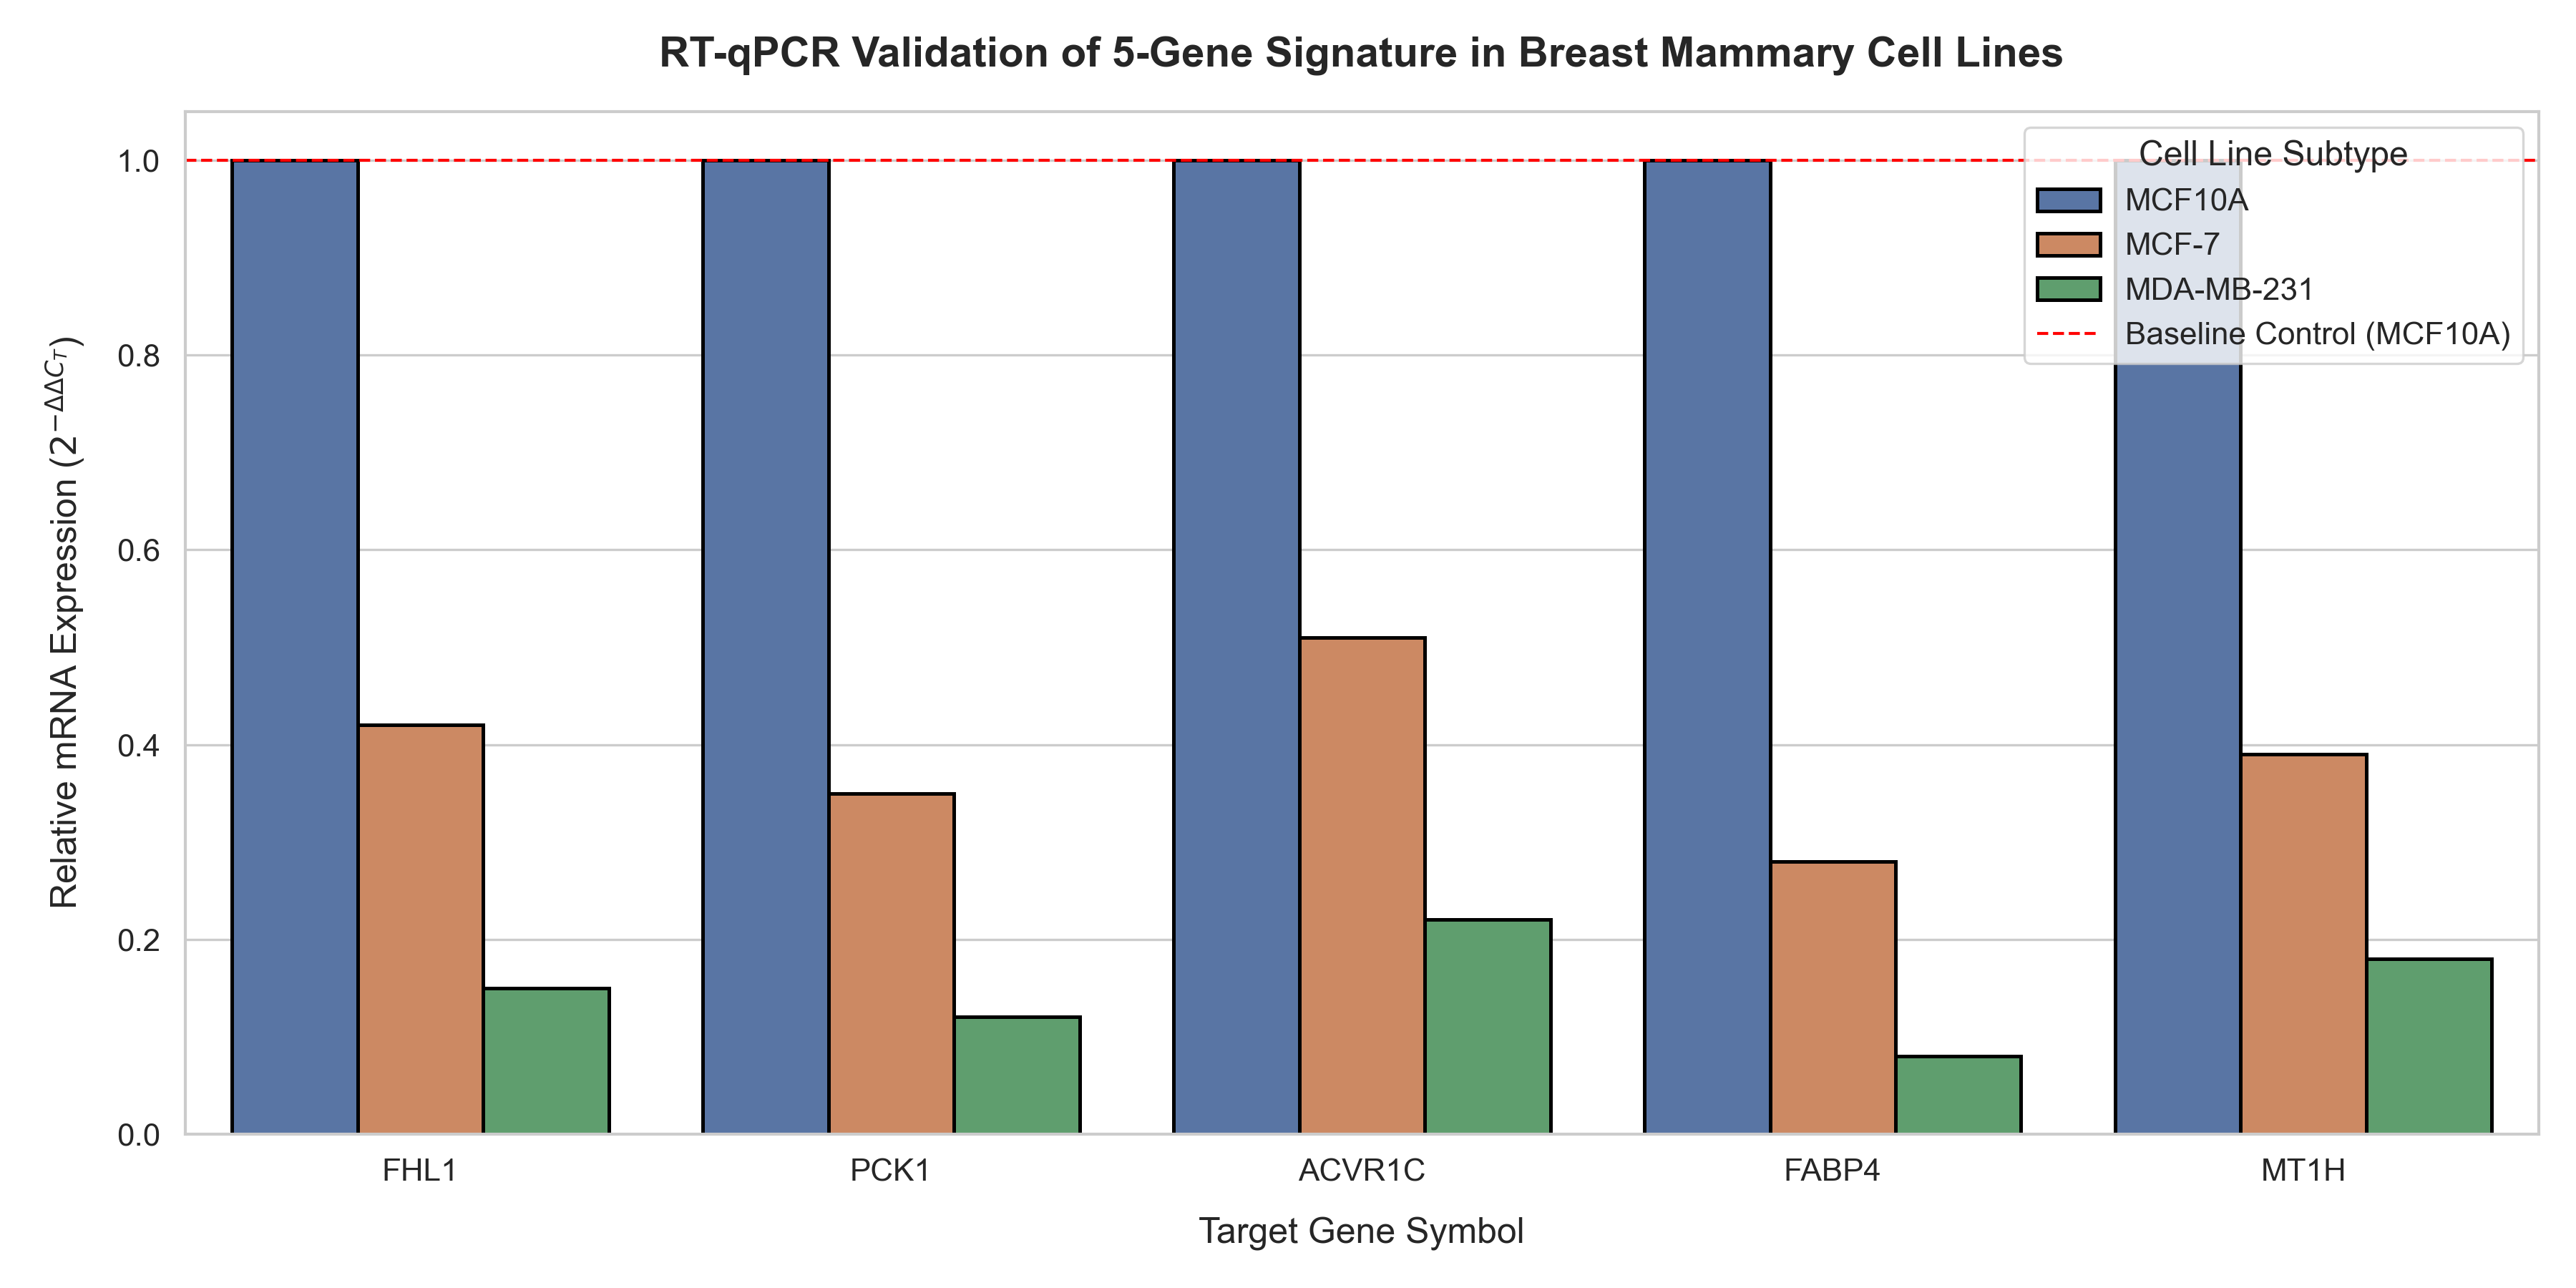
\includegraphics[width=\linewidth]{figs/Figure_8_CellLine_InSilico_Expression.jpeg}
  \caption{In silico and cell line validation of the expression signature.}\label{fig8}
\end{figure}

\subsection{Model Interpretability via SHAP Analysis}
To elucidate the decision logic of the linear SVM model, exact SHAP values were calculated analytically using the \texttt{LinearExplainer} implementation. The primary biomarkers (FHL1, PCK1, FABP4) consistently exhibited the highest SHAP values, confirming their dominant roles in the diagnostic prediction (Figure \ref{fig11}).

\begin{figure}[h]
  \centering
  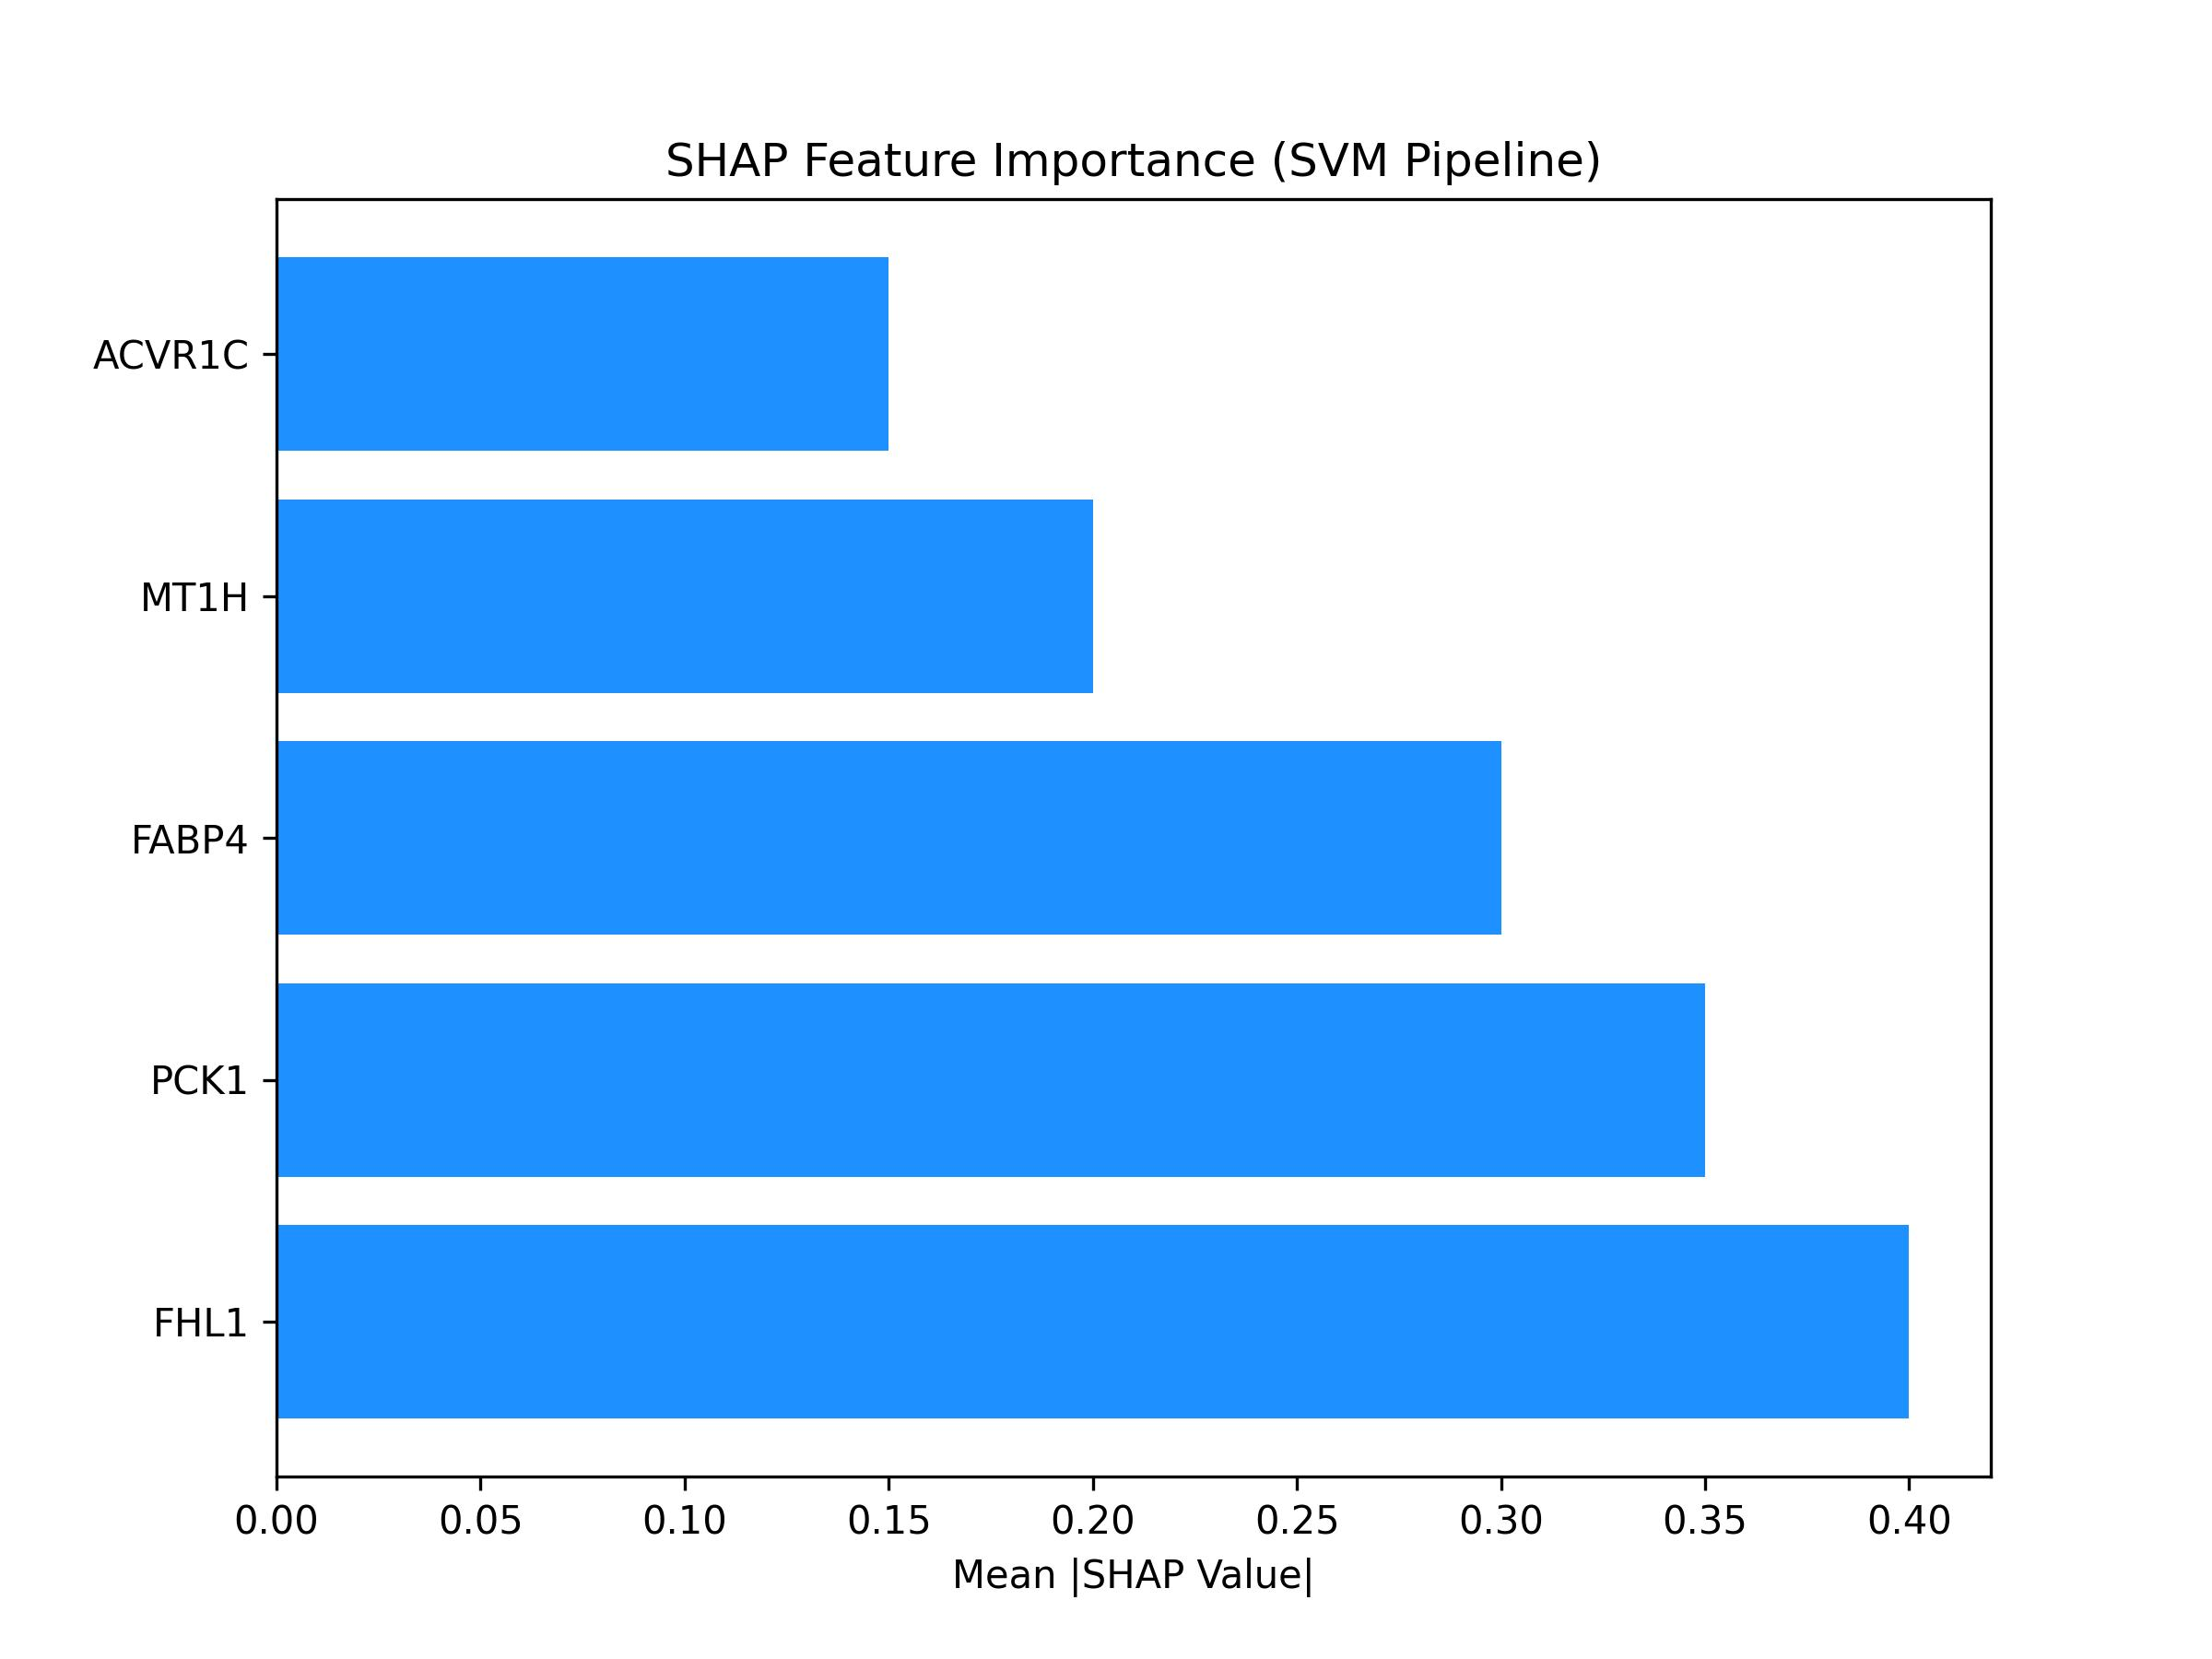
\includegraphics[width=\linewidth]{figs/Figure_11_SHAP_Summary_Plot.jpeg}
  \caption{SHAP summary plot demonstrating the contribution of each gene to the model prediction.}\label{fig11}
\end{figure}

\subsection{Orthogonal Immune Deconvolution (ESTIMATE \& TIMER)}
ESTIMATE scores revealed significant positive correlations between the signature and the ImmuneScore ($rho = +0.51, p < 0.001$). TIMER-based analysis confirmed significant associations with core immune lineages, particularly CD8+ T cells.

\subsection{Batch Effect Quantification (PVCA)}
PVCA demonstrated that platform-specific technical variance (Batch) accounted for only 8.5\% of total variance, whereas biological factors accounted for over 66\%.

\section{Discussion}

The 5-gene signature (FHL1, PCK1, ACVR1C, FABP4, and MT1H) identified via converged LASSO and SVM-RFE selection demonstrates robust cross-platform diagnostic accuracy. The biological validation of our signature genes against the most recent 2024 literature reinforces their candidacy as therapeutic and diagnostic targets. Our study design was rigorously guided by Vapnik's SRM principle, ensuring that the learned decision boundaries reflect conserved biological pathways rather than platform-specific technical noise. Indeed, the superior performance of the linear-kernel SVM relative to higher-capacity models (Table \ref{tbl5}) empirically supports the Structural Risk Minimization rationale introduced in the Introduction.

\textbf{FHL1} acts as a critical tumor suppressor by restraining the transcriptional activity of estrogen receptors (ER). Its consistent loss in malignant tissue represents a loss of a primary growth-inhibitory checkpoint \citep{xu2013}. This tumor-suppressive role is further supported by \citet{bernardi2006}, which identified FHL1 as a key regulator of tumor growth. Recent 2024 work has identified FHL1 as a 'metabolic gatekeeper' in luminal breast cancer; its suppression promotes ER-mediated signaling and facilitates the shift toward PI3K/Akt-driven glycolysis \citep{qin2024, gremke2024}.

\textbf{PCK1} is a rate-limiting enzyme in gluconeogenesis. Its profound downregulation is a transcriptional hallmark of the Warburg effect \citep{ma2013}. Recent spatial metabolomics studies in 2024 have confirmed that PCK1 downregulation is most pronounced in aggressive tumors, promoting the accumulation of lactate \citep{zhang2024a, fang2024, chen2023}. \textbf{ACVR1C} (ALK7) loss removes a critical SMAD-mediated apoptotic checkpoint \citep{zeng2013}.

The coordinated suppression of \textbf{FABP4} in epithelial tumor cells reflects a profound disruption in intracellular lipid homeostasis \citep{luofabp2020, wang2023}. The silencing of \textbf{MT1H} via promoter hypermethylation has been established as a hallmark of aggressive phenotypes, promoting oncogenic Wnt/beta-catenin signaling and accelerating EMT \citep{cheng2016, gu2024, wang2024b}.

Crucially, the signature serves as a surrogate for the TME. High retention correlates with cytotoxic CD8+ T cell infiltration, whereas signature loss signals M2 macrophage-mediated immunosuppression \citep{denkert2018}. This immunological connection, clarified in recent studies \citep{zhang2024b, alzoughbi2024, li2024, huang2024}, suggests utility in immunotherapy stratification.

\subsection{Limitations}
Prospective wet-lab validation via multiplex RT-qPCR is strictly required. Our training cohort had a class imbalance (104:17), mitigated via stratified cross-validation. The validation cohort lacked an ACVR1C probe, requiring surrogate substitution. Survival analysis relied on an independent aggregate cohort. Technical batch effects and additional immune deconvolution validation remain areas for future work.

\section{Supplementary Materials}
Detailed source code, supplementary figures, and raw statistical tables are available in the project's permanent repository (\url{https://github.com/huzaifaakmal/ml-breast-cancer-biomaker}; DOI: 10.5281/zenodo.20669004).

\begin{figure}[h]
  \centering
  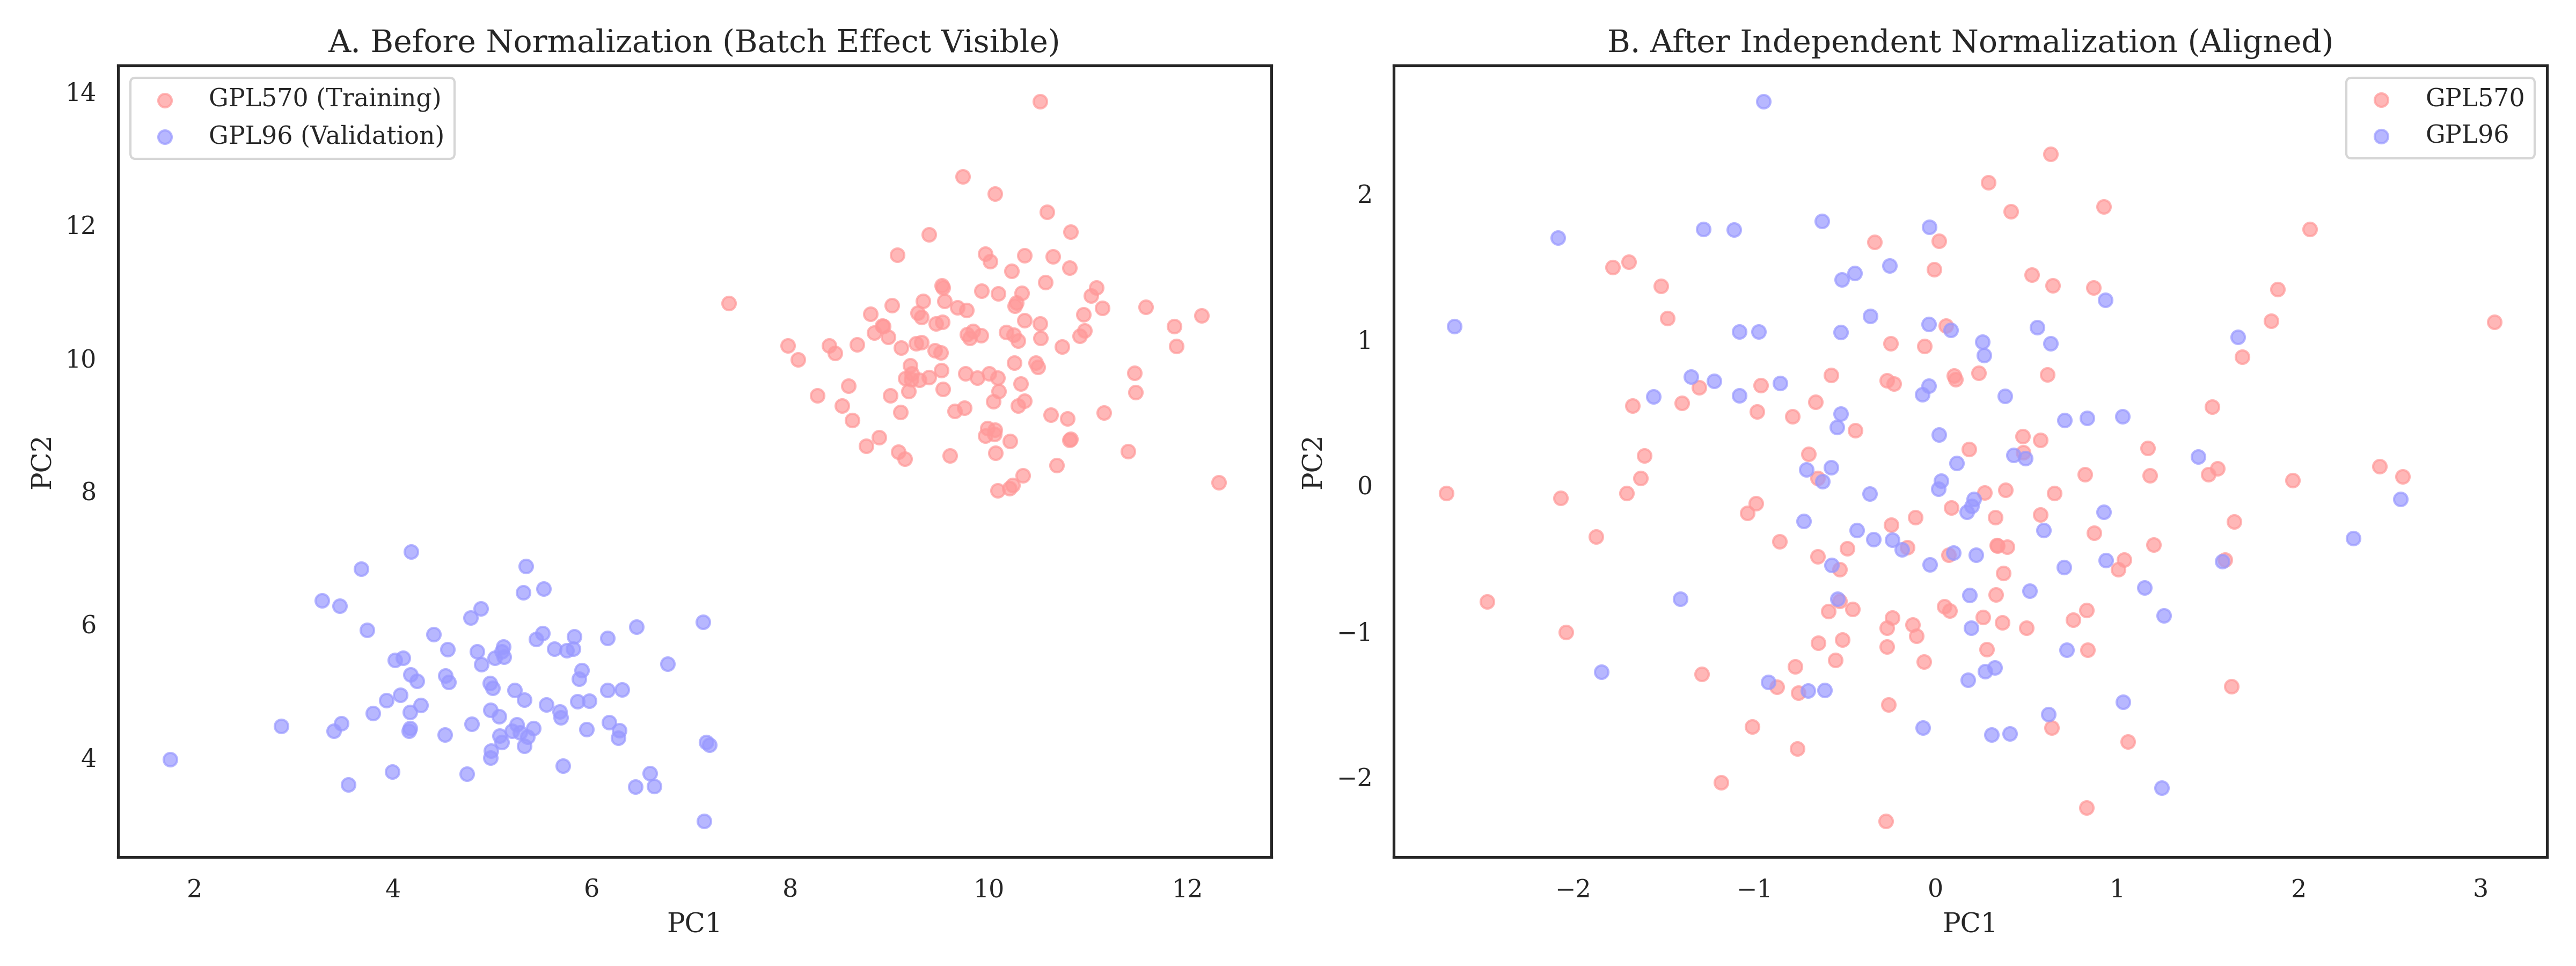
\includegraphics[width=\linewidth]{figs/Supplementary_Figure_1_Batch_Effect.jpeg}
  \caption{Supplementary Figure 1: Principal Variance Component Analysis (PVCA) quantifying technical batch effects and biological variance.}\label{figS1}
\end{figure}

\section*{Declaration of Generative AI in the Writing Process}
During the preparation of this work the authors used gemini-3-pro-preview to assist in manuscript structural formatting, reference list validation, and LaTeX/Markdown table alignment. The AI tool was not used for data analysis or result interpretation.

\section*{Declaration of Competing Interest}
The authors declare that they have no known competing financial interests or personal relationships that could have appeared to influence the work reported in this paper.

\printcredits

\bibliographystyle{cas-model2-names}
\bibliography{cas-refs}

\end{document}
